% \documentclass[fleqn,usenatbib]{mnras}
\documentclass[a4paper,11pt]{article}
% \pdfoutput=1
\usepackage{amsmath, amssymb}

\usepackage{jcappub}
\usepackage{newtxtext,newtxmath}
\usepackage[T1]{fontenc}
\usepackage{graphicx}
\usepackage{hyperref}
% \usepackage{amssymb}
% Allow "Thomas van Noord" and alike to be sorted by "N" etc. in the bibliography.
% Write the name in the bibliography as "\VAN{Noord}{Van}{van} Noord, Thomas"
\DeclareRobustCommand{\VAN}[3]{#2}
\let\VANthebibliography\thebibliography
\def\thebibliography{\DeclareRobustCommand{\VAN}[3]{##3}\VANthebibliography}

% martin comment function
\newcommand{\maf}[1]{{\textcolor{red}{[{\bf MAF}: #1]}}}
% mingfeng comment function
\newcommand{\mfh}[1]{{\textcolor{green}{[{\bf MFH}: #1]}}}
% simeon comment function
\newcommand{\spb}[1]{{\textcolor{magenta}{[{\bf SPB}: #1]}}}

% ming-feng emulator commands
\newcommand{\mfemu}{\texttt{MFEmulator}}     % i made the acronym, but not used a lot
\newcommand{\Data}{\mathcal{D}}
\newcommand{\gp}{\textsc{gp}}
\newcommand{\normal}{\mathcal{N}}
\newcommand{\GP}{\mathcal{GP}}
\newcommand{\thetavec}{\boldsymbol{\theta}}  % input parameters
\newcommand{\zvec}{\boldsymbol{z}}
\newcommand{\outputFunction}{Z}
\newcommand{\outputVector}{\zvec}            % output response
\newcommand{\outputVectorModel}{\zvec_\mathrm{model}}
\newcommand{\outputVectorObs}{\zvec_\mathrm{obs}}
\newcommand{\muvec}{\boldsymbol{\mu}}        % GP mean vector
\newcommand{\Kvec}{\boldsymbol{\mathrm{K}}}  % covariance matrix
\newcommand{\kvec}{\boldsymbol{k}}           % covariance vector
\newcommand{\Lya}{Lyman-$\alpha$}
\newcommand{\astrid}{\texttt{ASTRID}}
\newcommand{\nat}{Nature}

\newcommand{\uniform}{\mathcal{U}}

\newcommand{\apjs}{ApJ Supplement}
\newcommand{\apj}{ApJ}
\newcommand{\aap}{AAP}
\newcommand{\mnras}{MNRAS}
\newcommand{\prd}{PRD}
\newcommand{\gadget}{{\small GADGET}}
\newcommand{\mpgadget}{{\small MP-GADGET}}

\newcommand{\km}{k_{max}}

\newcommand{\vect}[1]
  {\mbox{\boldmath ${#1}$}}
\newcommand{\matr}[1]
  {\mbox{\bf \sf{#1}}}
\newcommand{\eq}[1]
  {Eq.~(\ref{equation:#1})}
\newcommand{\eqs}[1]
  {Eqs~(\ref{equation:#1})}
\newcommand{\sect}[1]
  {section~\ref{section:#1}}
\newcommand{\sects}[1]
  {sections~\ref{section:#1}}
\newcommand{\tabl}[1]
  {{\mbox Table~\ref{table:#1}}}
\newcommand{\tabls}[1]
  {{\mbox Tables~\ref{table:#1}}}
\newcommand{\fig}[1]
  {Fig.~\ref{Figure:#1}}
\newcommand{\figs}[1]
  {Figs.~\ref{Figure:#1}}
\newcommand{\sourcesection}[1]{\noindent {\em{#1}} ---}

\def\jcap{JCAP}        % Journal of Cosmology and Astro-Particle Physics

\newcommand{\Msun}{\, h^{-1} M_\odot}
\newcommand{\Zsun}{Z_\odot}
\newcommand{\NHunit}{cm$^{-2}$}
\newcommand{\sLLS}{\sigma_\mathrm{LLS}}
\newcommand{\Mpc}{\,\mathrm{Mpc}}
\newcommand{\Mpch}{\, h^{-1} \mathrm{Mpc}}
\newcommand{\kpch}{\, h^{-1}\mathrm{kpc}}
\newcommand{\hMpc}{\, h \mathrm{Mpc}^{-1}}
\newcommand{\kms}{km~s$^{-1}$}
\newcommand{\NHI}{N_\mathrm{HI}}

\newcommand{\edit}[1]{#1}

%opening
\title{A New Suite of Lyman-$\alpha$ Forest Simulations for Cosmology}

\author[a,1]{Martin Fernandez,\note{Corresponding author}}
\author[a]{Simeon Bird,}
\affiliation[a]{Department of Physics \& Astronomy, University of California  Riverside,\\900 University Avenue, Riverside, CA 92521, USA}
\author[b]{Others: Yueying, Tiziana, Nianyi, Yu? Rupert? Anson (for the hydrogen reionization boost)?}
\emailAdd{mfern027@ucr.edu}
\emailAdd{sbird@ucr.edu}

\abstract{
We present a new suite of $43$ simulations of the Lyman-$\alpha$ forest, spanning a $9$-dimensional parameter space, including $4$ cosmological parameters and $5$ astrophysical/thermal parameters. These simulations advance on earlier simulations suites by larger particle loads, by incorporating new physical models for hydrogen and helium reionization, and by self-consistently incorporating a model for AGN feedback. Parameters are chosen based on a Latin hypercube design and a Gaussian process is used to interpolate to arbitrary parameter combinations. Our simulation suite will be used to interpret existing Lyman-$\alpha$ forest 1D flux power spectra from SDSS and future DESI data releases.
}

\begin{document}

\maketitle

\section{Introduction}

Introduce the problem. Cite the previous simulation suites for the Lyman alpha forest. The purpose of a simulation suite is to compare to observational measurements. The main output of our suite is a set of medium resolution artificial flux power spectra, from which the flux power spectrum may be generated. In this paper we describe the simulation suite we have run and defer description of the likelihood function to upcoming work.

\section{Simulations}

Overall, we have performed $43$ cosmological hydrodynamic simulations, varying $9$ cosmological and astrophysical parameters. Each simulation contains $1536^3$ gas particles and $1536^3$ cold dark matter particles and models a $120$ Mpc/h periodic box. These choices are justified in Section~\ref{sec:boxsize}. Simulations were run using \mpgadget~\cite{MPGadget2018, Bird:2022}, a massively scalable version of the cosmological structure formation code Gadget-3 \cite{Springel:2005}. The generation of initial conditions is described in Section~\ref{sec:initconds}. Section~\ref{sec:gravity} describes the gravity solver, hydrodynamic solver, and cooling.

Sections~\ref{sec:hydrogen} and ~\ref{sec:helium} describe our models for hydrogen and helium reionization respectively, and how their parameters map to the familiar thermal parameters of the \Lya~forest. We have chosen to vary the parameters of our hydrogen and helium reionization models in order to model uncertainty in the thermal history of the intergalactic medium (IGM).
A wide variety of earlier models instead generate arbitrary thermal histories by scaling the heating rates directly \cite[e.g.~][]{Viel:2006}. Scaling the heating rates allows the greatest possible freedom in the redshift evolution of the thermal histories, but does does not directly impose a physically plausible thermal history, which can sometimes lead to best-fit thermal histories which do not correspond to actual simulations \cite{Walther:2019}, Conversely, Ref.~\cite{Garzilli:2021} \spb{I think this may be Garzilli 2019} argued that the assumption of a power law evolution of the mean temperature with redshift \cite{Viel:2013wdm, Irsic:2017} provides a strong prior, although see \spb{Cite the next Viel paper and Garzilli paper} where stronger data validated the original thermal evolution. Constraining the parameters of physical reionization models ensures that the redshift evolution of the thermal histories produced are physically plausible and self-consistent, and thus simplifies our inference. This choice is enabled by two advances: first, our simulation boxes are large enough to contain many helium reionization bubbles and second, the thermal history of the IGM is now reasonably well constrained, limiting the variety of models it is necessary to marginalise over.

We use a suite of full physics simulations including star formation, stellar winds and AGN feedback. We use full physics simulations primarily because it allows us to incorporate our AGN feedback model self-consistently into the code, rather than with a post-processing correction. AGN feedback has been shown to influence the \Lya~forest flux power spectrum \cite{Viel:2013, Chabanier:2020}. Full-physics simulations also allow us to self-consistently include the effect of self-shielded gas in the modelling, by producing DLAs in our spectral code and removing them, as in the observational analysis. We stress that these are likely small effects and we do not wish to imply that quick \Lya~models are inadequate for current data. However, with current simulation codes the speed difference between the quick \Lya~and full physics simulations is only $\sim 30\%$, and so the cost is relatively small. Furthermore, using full physics simulations allows our suite to be used for other applications in future.

Our galaxy formation model parameters generally follow those used in the \astrid~simulation, as detailed in Refs.~\cite{Bird:2022, Ni:2021}. Here we summarise the main features of the model, and refer the interested reader to \cite{Bird:2022} for more details. Readers familiar with \astrid~should refer to Table~\ref{tab:paramchanges}, which summarises the differences in the galaxy formation model. We describe the star formation and stellar wind model in Section~\ref{sec:stellar}, and the black hole and AGN feedback model in Section~\ref{sec:agn}.

\begin{table*}
\begin{centering}
  \begin{tabular}{lll}
  \hline
  Parameter & New Value & \astrid~Value \\
    \hline
SPH density kernel  & Cubic & Quintic \\
Minimum wind velocity $v_w$ & $100$ km/s & $0$ \\
Temperature at HI reionization & $15000$ K & $0$ K \\
Stars per gas particle & $1$ & $4$ \\
Metal return from stars & Disabled & Enabled\\
Metal line cooling & Disabled & Enabled. \\
    \hline
  \end{tabular}
  \caption{Summary of changes and simplifications in the galaxy formation model from the \astrid~simulation.}
  \label{tab:paramchanges}
  \end{centering}
\end{table*}

%The initial conditions include separate transfer functions for baryons and cold dark matter. The initial distribution of cold dark matter particles is a grid, and the initial distribution of baryons is a Lagrangian glass, as recommended by \cite{Bird:2020} to reduce particle transients. First-order Lagrangian perturbation theory \citep{Zeldovich:1970, Crocce:2006} is used to initialise particle positions and velocities. Second-order terms are not included as they are difficult to model when the initial transfer functions for baryons and cold dark matter are different. Radiation density is included in the cosmological background evolution.
%, a $10\%$ contribution to the Hubble expansion at $z=100$ that affects the total integrated growth rate at the $10\%$ level by $z=10$.

\subsection{Initial Conditions}
\label{sec:initconds}

Cosmological parameters and prior ranges are:
\begin{align}
      n_s      &\sim \uniform[0.8, 0.995]; \\
      A_P      &\sim \uniform[1.2\times10^{-9}, 2.6\times10^{-9}];\\
      h        &\sim \uniform[0.65, 0.75]; \\
      \Omega_0 h^2 &\sim \uniform[0.14, 0.146];\\
   \label{eq:prior_cos_volume}
\end{align}
$A_p$ is the amplitude of perturbations at $k = 0.78$ h/Mpc, chosen to be in the middle of the range probed by the \Lya~forest and thus reduce artificial correlation between $n_s$ and $A_P$ \cite{Bird:2019}. $n_s$ is the spectral index. The primordial power spectrum is thus:
\begin{equation}
 P(k) = A_P \left(\frac{k}{ 0.78}\right)^{n_s-1}\,.
 \label{eq:pk}
\end{equation}
We have chosen the prior ranges for $A_P$ to include the posterior constraint from Planck, measured on larger scales \cite{Planck:2018}.
%This pivot scale is not the same as used in the CMB and thus scalar amplitude $A_P$ is not directly comparable to $A_s$ as measured on larger scales. However, w
$h$ is the Hubble parameter, and $\Omega_0 h^2$ controls the growth rate. We do not vary $\Omega_b$ as it is degenerate with the ionization fraction of the gas. It is not necessary to include an explicit parameter for neutrino mass as the effect of neutrino mass on the forest is degenerate with $A_P$. Schematically, neutrino mass constraints come from measuring different power spectrum amplitudes on CMB and \Lya~scales \cite{Pedersen:2021}.

In practice both $h$ and $\Omega_0 h^2$ do not strongly influence the final \Lya~forest posteriors in our current analysis, and so is not strongly constrained by the \Lya~forest.


\subsection{Gravity, Hydrodynamics and Cooling}
\label{sec:gravity}

%The gravity solver in MP-Gadget uses the same basic algorithms as Gadget-3.
We use the same gravity solver described in Ref.~\cite{Bird:2022} and references therein. Long range gravitational forces are computed in Fourier space using a particle-mesh algorithm. Short-range forces, below the resolution of the particle grid, are computed using a hierarchical multipole expansion of the gravitational field, leading to a uniformly high force resolution throughout the computational volume. The default accuracy of the split between short and long range forces has been increased and the force accuracy of \mpgadget~is better than 1\% as measured against an exact N-body solver.
%able to reproduce the matter power spectrum output by PKDGRAV3 to $<1\%$ \cite{Schneider:2016}.

We adopt the pressure-entropy formulation of smoothed particle hydrodynamics (pSPH) to solve the Euler equations \citep{Hopkins:2013,Read:2010} as implemented by \cite{Feng:2014}. %The density estimator uses a quintic density kernel to reduce noise in SPH density and gradient estimation \citep{2012JCoPh.231..759P}.
The SPH density kernel uses a cubic polynomial, rather than the quintic kernel from \astrid, as the reduced number of neighbours improves resolution in the \Lya~forest. This comes at the cost of increased noise in dense regions, but at forest densities this does not affect the dynamics \cite{Bird:2013}.
Gas is allowed to cool radiatively following \citep{Katz:1996}.
We have used the updated cooling coefficients summarised in \cite{Bolton:2017}, the recombination rates from \cite{Verner:1996} and collisional ionization rates from \cite{Voronov:1997}. Self-shielding of neutral hydrogen is included following the fitting function of \cite{Rahmati:2013}.
The UV background used is the ``optically thin'' variant from Ref.~\cite{FG2020}. There is also a variant which corrects for the average effect of partial reionization on the gas temperature; we do not use this as we instead include explicit models for patchy reionization.

\subsection{Hydrogen Reionization}
\label{sec:hydrogen}

We model patchy reionization with a spatially varying ultra-violet background using a semi-analytic method \cite{Battaglia:2013} which pre-computes a reionization redshift, on a grid with cells $1$ Mpc/h, using FASTPM \cite{FASTPM}. The redshift of reionization, $z_{HI}$, is defined as the redshift at which $50\%$ of the simulation volume has reionized. In general, higher initial overdensities reionize earlier.

For gas particles in a region which has not yet reionized, the photon background is set to zero and the gas remains neutral. Once the reionization redshift has passed, the particle's ionization and thermal states evolve in ionization equilibrium with the external UV background. Newly in these simulations, we include a temperature boost to each gas particle as it passes the reionization redshift to account for the (subgrid) heating effect of ionization fronts.
Each gas particle on reionization has its temperature boosted to $15,000$K.
Ref.~\citep{DAloisio:2019} found a temperature boost of $\sim 20,000$K in their radiative transfer simulations. However, our simulation is much lower resolution and has much longer timesteps, suggesting that we should expect a certain amount of subgrid cooling before any given particle in our simulation box becomes active. Furthermore, we found that a temperature boost of $20,000$ K led to generally higher IGM temperatures when compared to observations $z\sim 6$, at least for the relatively low reionization redshifts preferred by current mean free path observations \cite{Cain:2021}.

The reionization temperature boost means that $z_{HI}$ affects the thermal history of the IGM. After reionization the UV background is not sufficiently intense to preserve a thermal equilibrium and so the gas cools. The reionization parameter, $z_{HI}$, thus controls the IGM temperature before helium reionization starts at at $z \gtrsim 4$.

Note that as long as $z_{HI} > 5.8$, the current highest redshift IGM temperature measurement \cite{Gaikwad:2021?}, $z_{HI}$ is observationally degenerate with the size of the reionization temperature boost. Our ultimate constraints on the reionization redshift should thus be understood to be conditional on a boost of $15,000$ K.

%We do not boost the gas temperature to account for the passage of ionization fronts \citep{2019ApJ...874..154D}.

\subsection{Helium Reionization}
\label{sec:helium}

We include a model for spatially inhomogeneous helium reionization following \cite{UptonSanderbeck:2020}. Reionized bubbles are placed around randomly chosen halos with mass $M_{\rm halo}\geq 10^{12}$M$_{\odot}$, a mass range chosen to have a reasonable chance of hosting a quasar. Bubbles are $20$ Mpc/h across, matching the mean bubble size found in radiative transfer simulations \citep{McQuinn:2009}. Inside this bubble a quasar radiation field is assumed with a spectral index of $- \alpha_q$, which we vary in our simulation suite. During the reionization timestep gas particles in a bubble are abruptly heated and marked as ionized. Should bubbles overlap, only particles not already marked as ionized are heated. Bubbles are placed until the total ionized gas mass in the box reaches
\sob{...}

Thermal histories are marginalised by varying the free parameters of the model, described in Eq.~\ref{eq:prior_reion_volume}. Reionized bubbles of $20$ Mpc/h across are placed around randomly chosen quasar-hosting halos, matching the results of radiative transfer simulations \citep{McQuinn:2009}.

Our model includes the patchiness of helium reionization and the resulting fluctuations in temperature, ionization state, and pressure smoothing. A consequence is that there is no unique temperature-density relation in our simulations, but a range of temperature-density relations depending on the time at which a given part of the simulation reionized.

The distribution of \Lya~forest gas is influenced by the temperature and temperature-density relation of the IGM.
\begin{align}
      z_{Hei}        &\sim \uniform[3.5, 4.1]; \\
      z_{Hef}        &\sim \uniform[2.6, 3.2]; \\
      \alpha_q      &\sim \uniform[1.6, 2.5]; \\
      z_{Hi}        &\sim \uniform[6.5, 8]; \\
   \label{eq:prior_reion_volume}
\end{align}

$z_{Hei}$ and $z_{Hef}$ are the start and end redshifts, respectively, of helium reionization. $z_{Hi}$ is the midpoint redshift of hydrogen reionization. $\alpha_q$ is the quasar emissivity spectral index, which controls the peak IGM temperature at the midpoint of helium reionization.

\begin{table*}
\begin{centering}
  \begin{tabular}{llll}
  \hline
  Parameter & Minimum & Maximum & Description \\
    \hline
    $n_s$  &  $0.8$  & $0.995$ & Scalar spectral index \\
    $A_P$  &  $2.2 \times 10^{-9}$  & $2.6 \times 10^{-9}$ & Power amplitude at $k = 0.78$ h/Mpc \\
    $h$    & $0.65$  & $0.75$ & Hubble parameter \\
    $\Omega_0 h^2$ & $0.14$ & $0.146$ & Total matter density \\
    $z_{Hei}$      & $3.5$  & $4.1$  & Start redshift of HeII reionization \\
    $z_{Hef}$      & $2.6$  & $3.2$  & End redshift of HeII reionization \\
    $\alpha_q$     & $1.6$  & $2.5$ & Quasar spectral index during HeII reionization  \\
    $z_{Hi}$        & $6.5$ & $8$   & Median redshift of HI reionization \\
    $\epsilon_{AGN}$ & $0.03$ & $0.07$ & Thermal efficiency of black hole feedback \\
    \hline
  \end{tabular}
  \caption{Summary of varied emulator parameters, together with the ranges covered by the emulator. We vary a total of $9$ parameters: $4$ for cosmology, $3$ for the helium reionization model, $1$ for the hydrogen reionization model and $1$ for the strength of AGN feedback.}
  \label{tab:emulatorparams}
  \end{centering}
\end{table*}

\subsection{Star Formation and Stellar Feedback}
\label{sec:stellar}

Stars form on an effective equation of state in dense gas, following \cite{Springel:2003}. Stars are formed with the same mass as a gas particle, so that gas particles are converted directly to stars. Note that \astrid~formed stars with $1/4$ of the mass of the gas particle. This increases the number of particles in dense regions which have little effect on the \Lya~forest, and so for our simulation suite simply increases computational cost.

We disable metal return from stars, as evaluating this model can be computationally expensive, and we are building an emulator for the neutral hydrogen of the \Lya~forest. We also disable metal cooling, which Ref.~\cite{Viel:2013} showed has a small effect on the \Lya~forest flux power spectrum. Similarly, we do not include the (metallicity dependent) correction to the high redshift star formation rate due to the formation of molecular hydrogen implemented in \astrid, which has a very small effect for $z < 6$.

A stellar wind feedback model is included following Ref.~\citep{Okamoto:2010} and Ref.~\cite{Bird:2022}. Wind speeds are proportional to the local one dimensional dark matter velocity dispersion $\sigma_\mathrm{DM}$:
\begin{equation}
v_w = \kappa_w \sigma_\mathrm{DM} \,,
\end{equation}
where $v_w$ is the wind speed. $\kappa_w$ is a dimensionless parameter, which we take to be $3.7$ following \cite{Vogelsberger:2013}. We have mildly altered the model from \cite{Bird:2022} by implementing a minimum wind velocity, $v_w \geq 100$ km/s, in order to improve convergence with resolution.

Winds are sourced by newly formed star particles, which randomly pick gas particles from within their SPH smoothing length to become wind particles. The total mass loading is $(v_w/ 350 \mathrm{km/s})^{-2}$ where $350$ km/s is in physical units. Particles recouple when their surrounding density drops by a factor of $10$, or after $60$ Myr.\footnote{In Ref.~\cite{Bird:2022} we had a subdominant recoupling condition: gas would recouple after $20 \mathrm{kpc} / v_w$. In practice this affected only a small fraction of the wind, as for a typical star forming halo with a virial velocity of $200$ km/s the recoupling time was $100$ Myr, and gas always recoupled after $60$ Myr. We have thus removed this condition for model simplicity.} Particles in the wind cool, but do not experience or produce pressure forces, nor may they be accreted onto a black hole. However, to enhance the stability of the SPH density estimates, they are included when computing SPH smoothing lengths.

We conducted an early test emulator using small boxes where the dimensionless supernova wind velocity, $\kappa_w$, was a free parameter of the model. However, we found that this free parameter was essentially unconstrained by the \Lya~forest data and so opted not to vary it in the full emulator run. Ref.~\cite{Bolton:2017} showed that supernova winds increased the \Lya~flux power on large scales, $k < 10^{-2}$ s/km, at $z < 3$, by around $10\%$, due to the presence of additional high column density systems\footnote{Ref.~\cite{Viel:2013} found that the \Lya~flux power spectrum was increased only for $ k > 0.04$ s/km (scales smaller than those measured by BOSS), but their simulations did not include self-shielding and so did not contain high column density absorbers.}. We remove high column density systems from our simulated spectra to match the observational procedure, and thus changes to the supernova wind model do not affect the \Lya~flux power spectrum. As shown in Figure~\ref{fig:DLACDDF}, our supernova simulation model parameters have been chosen to match the observed galaxy stellar mass function and thus the distribution of high column density absorbers. This good agreement can be taken as a strong prior on the supernova wind parameters and justifies our choice to fix the wind model in our emulator.

\begin{figure*}
% \includegraphics[width=1.\textwidth]{figures/cddf.pdf}
 \caption{CDDF of high column density absorbers from our simulation at $z=2$.}
 \label{fig:DLACDDF}
\end{figure*}

\subsection{AGN Feedback}
\label{sec:agn}

We include the effect of thermal AGN feedback in our simulations. We use the model of AGN feedback described in Ref.~\cite{Bird:2022}

Ref.~\cite{Viel:2013} showed an effect of AGN feedback which rises to $10\%$ at $z=2$, while Ref.~\cite{Chabanier:2020} found $8\%$ at $z=2$ and $k = 0.005$ s/km. Both simulations use AGN feedback models with parameters tuned to match the properties of galaxies at $z=0$. However, the implementations are different. Ref.~\cite{Chabanier:2020} uses the Horizon-AGN simulation \cite{Dubois:2016}. The AGN feedback model has two modes, one thermal and one kinetic, with the kinetic mode dominating at low accretion rates. Ref.~\cite{Viel:2013} uses the OWLS simulation suite, and delivers AGN feedback energy thermally, once black hole accretion has accumulated enough energy to heat a nearby gas particle to $10^8$ K. Despite the different implementations, the two codes agree reasonably well as to the effect of AGN feedback on the \Lya~forest.

\cite{Giri:2021} show that the effect is well described by the halo scale at which AGN feedback starts to remove the gas.

%Since the level of AGN feedback present in simulations is currently uncertain, we vary the strength of thermal feedback in our emulator.

This allows us to ensure that potential parameter degeneracies between AGN feedback and cosmological parameters are included. Ref~\cite{Schneider:2015} has shown that the main degeneracy for the matter power spectrum is between AGN feedback and the fraction of matter in baryons, $\Omega_b / \Omega_0$, as the AGN feedback . However, our main observable is the \Lya~forest which is sensitive to the thermal state of the gas and thus the heating effect of the AGN feedback as well as its ability to remove gas from the halo may be relevant.

\spb{Plot of the effect of the AGN feedback parameter. Ideally I would compare this to the correction factor from Chabanier et al.}
$\epsilon_{AGN} \sim \uniform[0.03, 0.07]$

\begin{figure*}
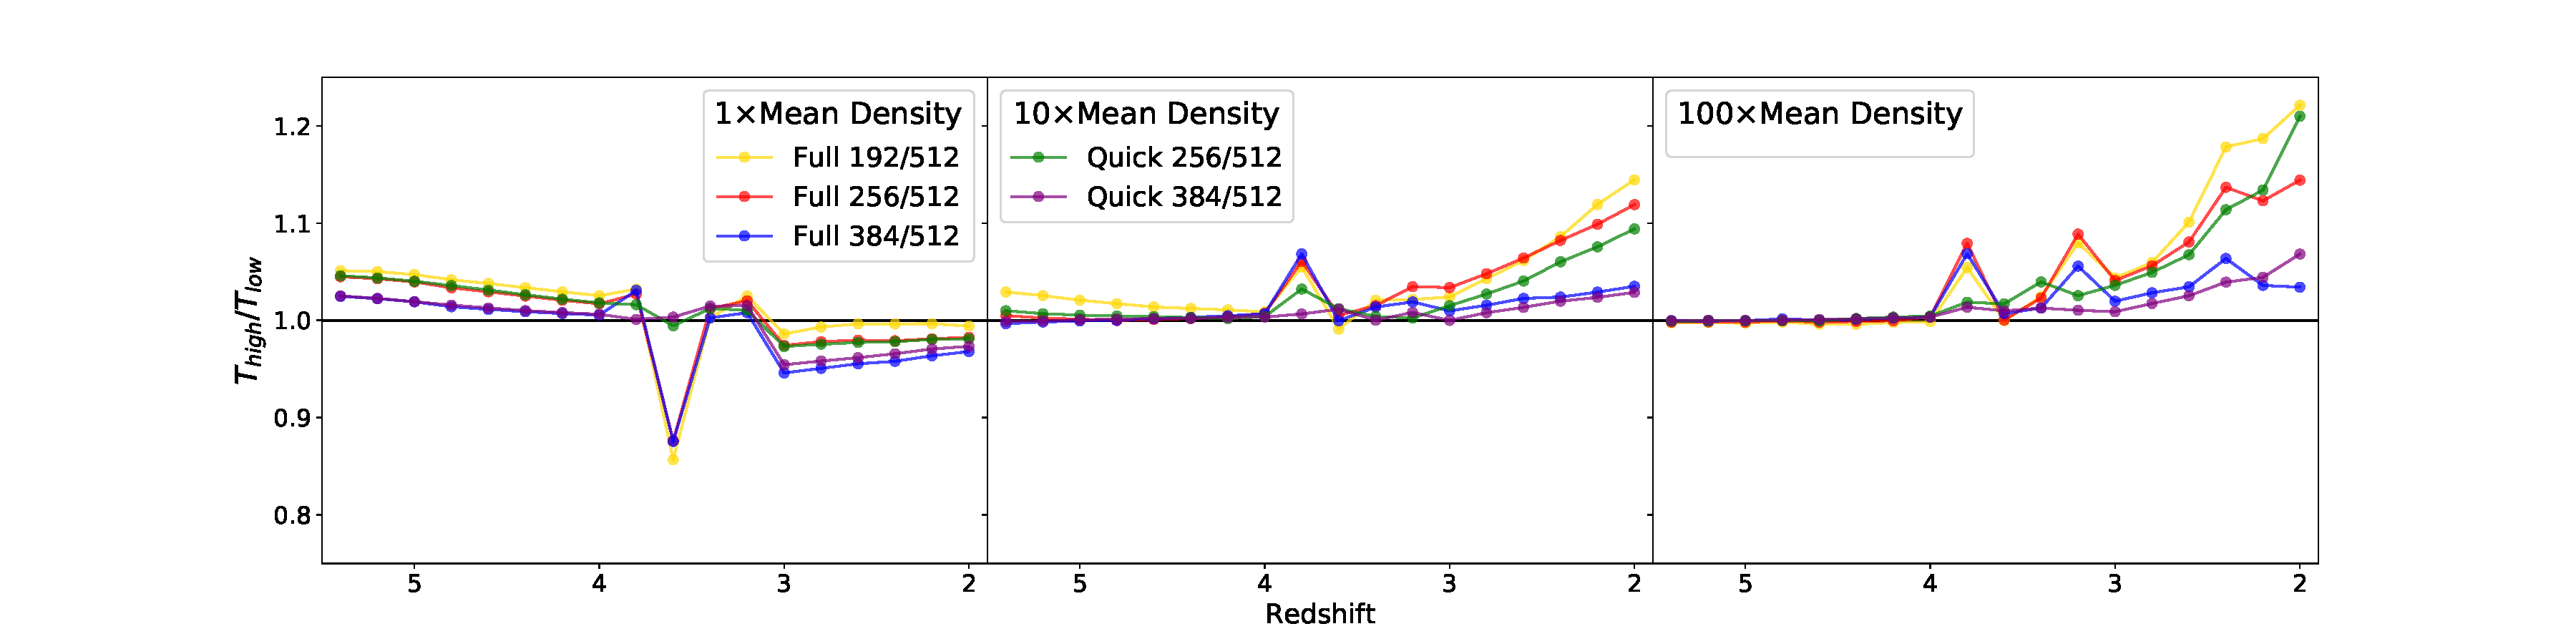
\includegraphics[width=1.\textwidth]{figures/comp-temps_fq.pdf}
 \caption{Temperature variations at different densities for different AGN feedback strengths. Make the point that higher densities are more affected by AGN feedback.}
 \label{fig:AGNtemp}
\end{figure*}

\subsection{Experimental Design}

% Describe the chosen cosmological parameters. Add a plot as Figure 3 of the multi-fidelity paper. Explain why these parameters are chosen. We use a Latin Hypercube design. Outputs are every $\Delta z=0.2$ from $z=5.4$ to $z=2.0$.

We vary a total of $9$ parameters. These include $4$ cosmological parameters, $3$ parameters for the helium reionization model, $1$ parameter for hydrogen reionization, and $1$ parameter for the strength of AGN feedback.

\spb{Latin hypercube design and Bayesian optimisation. Parameters which do not really influence the \Lya~forest are basically free with a LH.}

%Note that the emissivity is as $-\alpha_q$, so that larger values indicate a lower maximum IGM temperature.

Our emulator includes two additional parameters, modelled by post-processing spectra, are $2$ parameters for the amplitude of the uncertain mean optical depth in the \Lya~forest, $\tau_0$ and derivative $d\tau_0$, varying as a power law \spb{Copy from older emulator paper} As these parameters can be included in post-processing, they do not require extra simulations, but they are included as input parameters in our emulator. Note that our emulator is constructed so that we could easily use more general forms for the redshift variation of the mean optical depth if supported by observational data. \spb{Describe sampling}

\begin{figure}
    \centering
	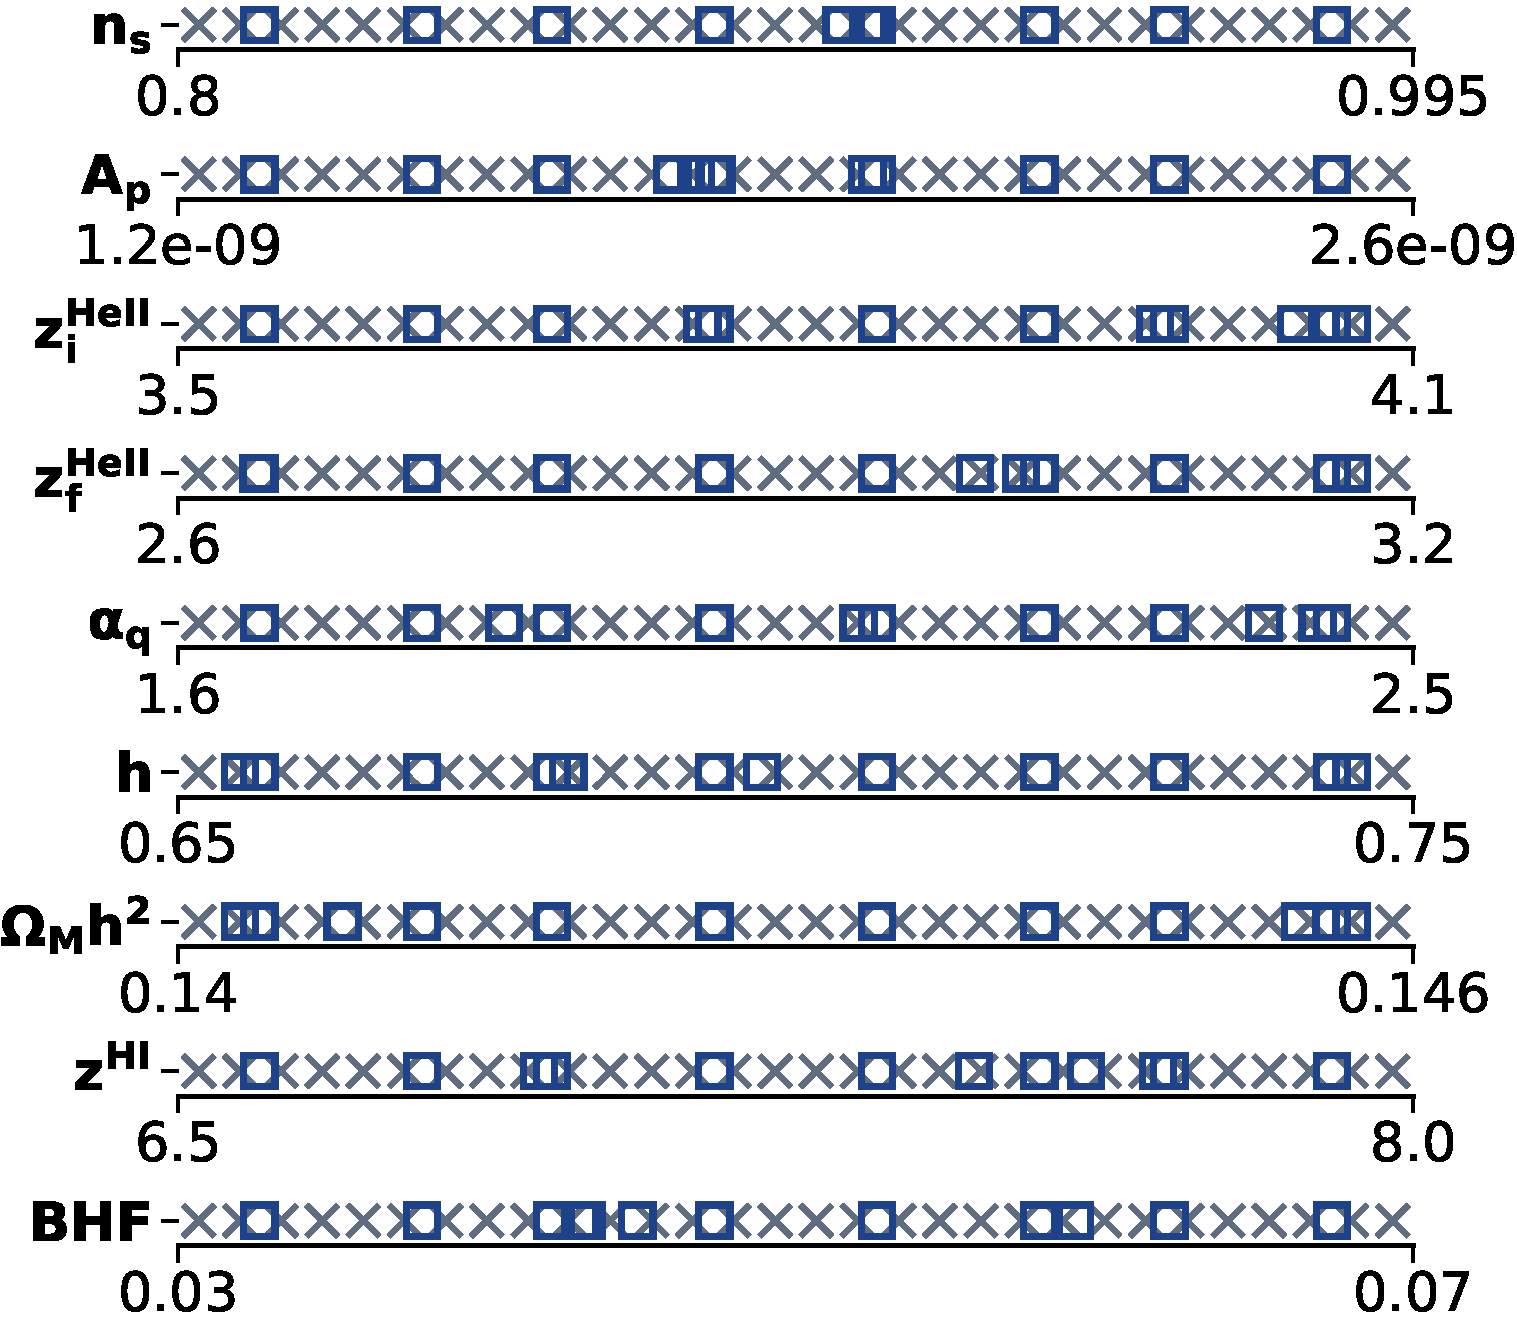
\includegraphics[width=0.5\columnwidth]{figures/120box_42samples.pdf}
    \caption{Simulation parameter limits, and samples used to construct the emulators presented. Shown as crosses are the initial Latin hypercube simulations, while the squares are the
    Parameters for the low resolution simulations (crosses) were determined by filling a Latin hypercube.
    From the low resolution set, the optimal high resolution set is determined, and these are shown as red circles.
    Initially, $30$ low resolution samples were generated, then an additional $10$ were added while maintaining the Latin hypercube method, hence the non-uniform spacing for the low resolution samples. \spb{Martin please remake}}
    \label{fig:samples}
\end{figure}

The emulator construction follows \cite{Bird:2019}.

\section{Results}

Plots of the effect of each parameter on the flux power spectrum from the emulator.

\begin{figure}
    \centering
	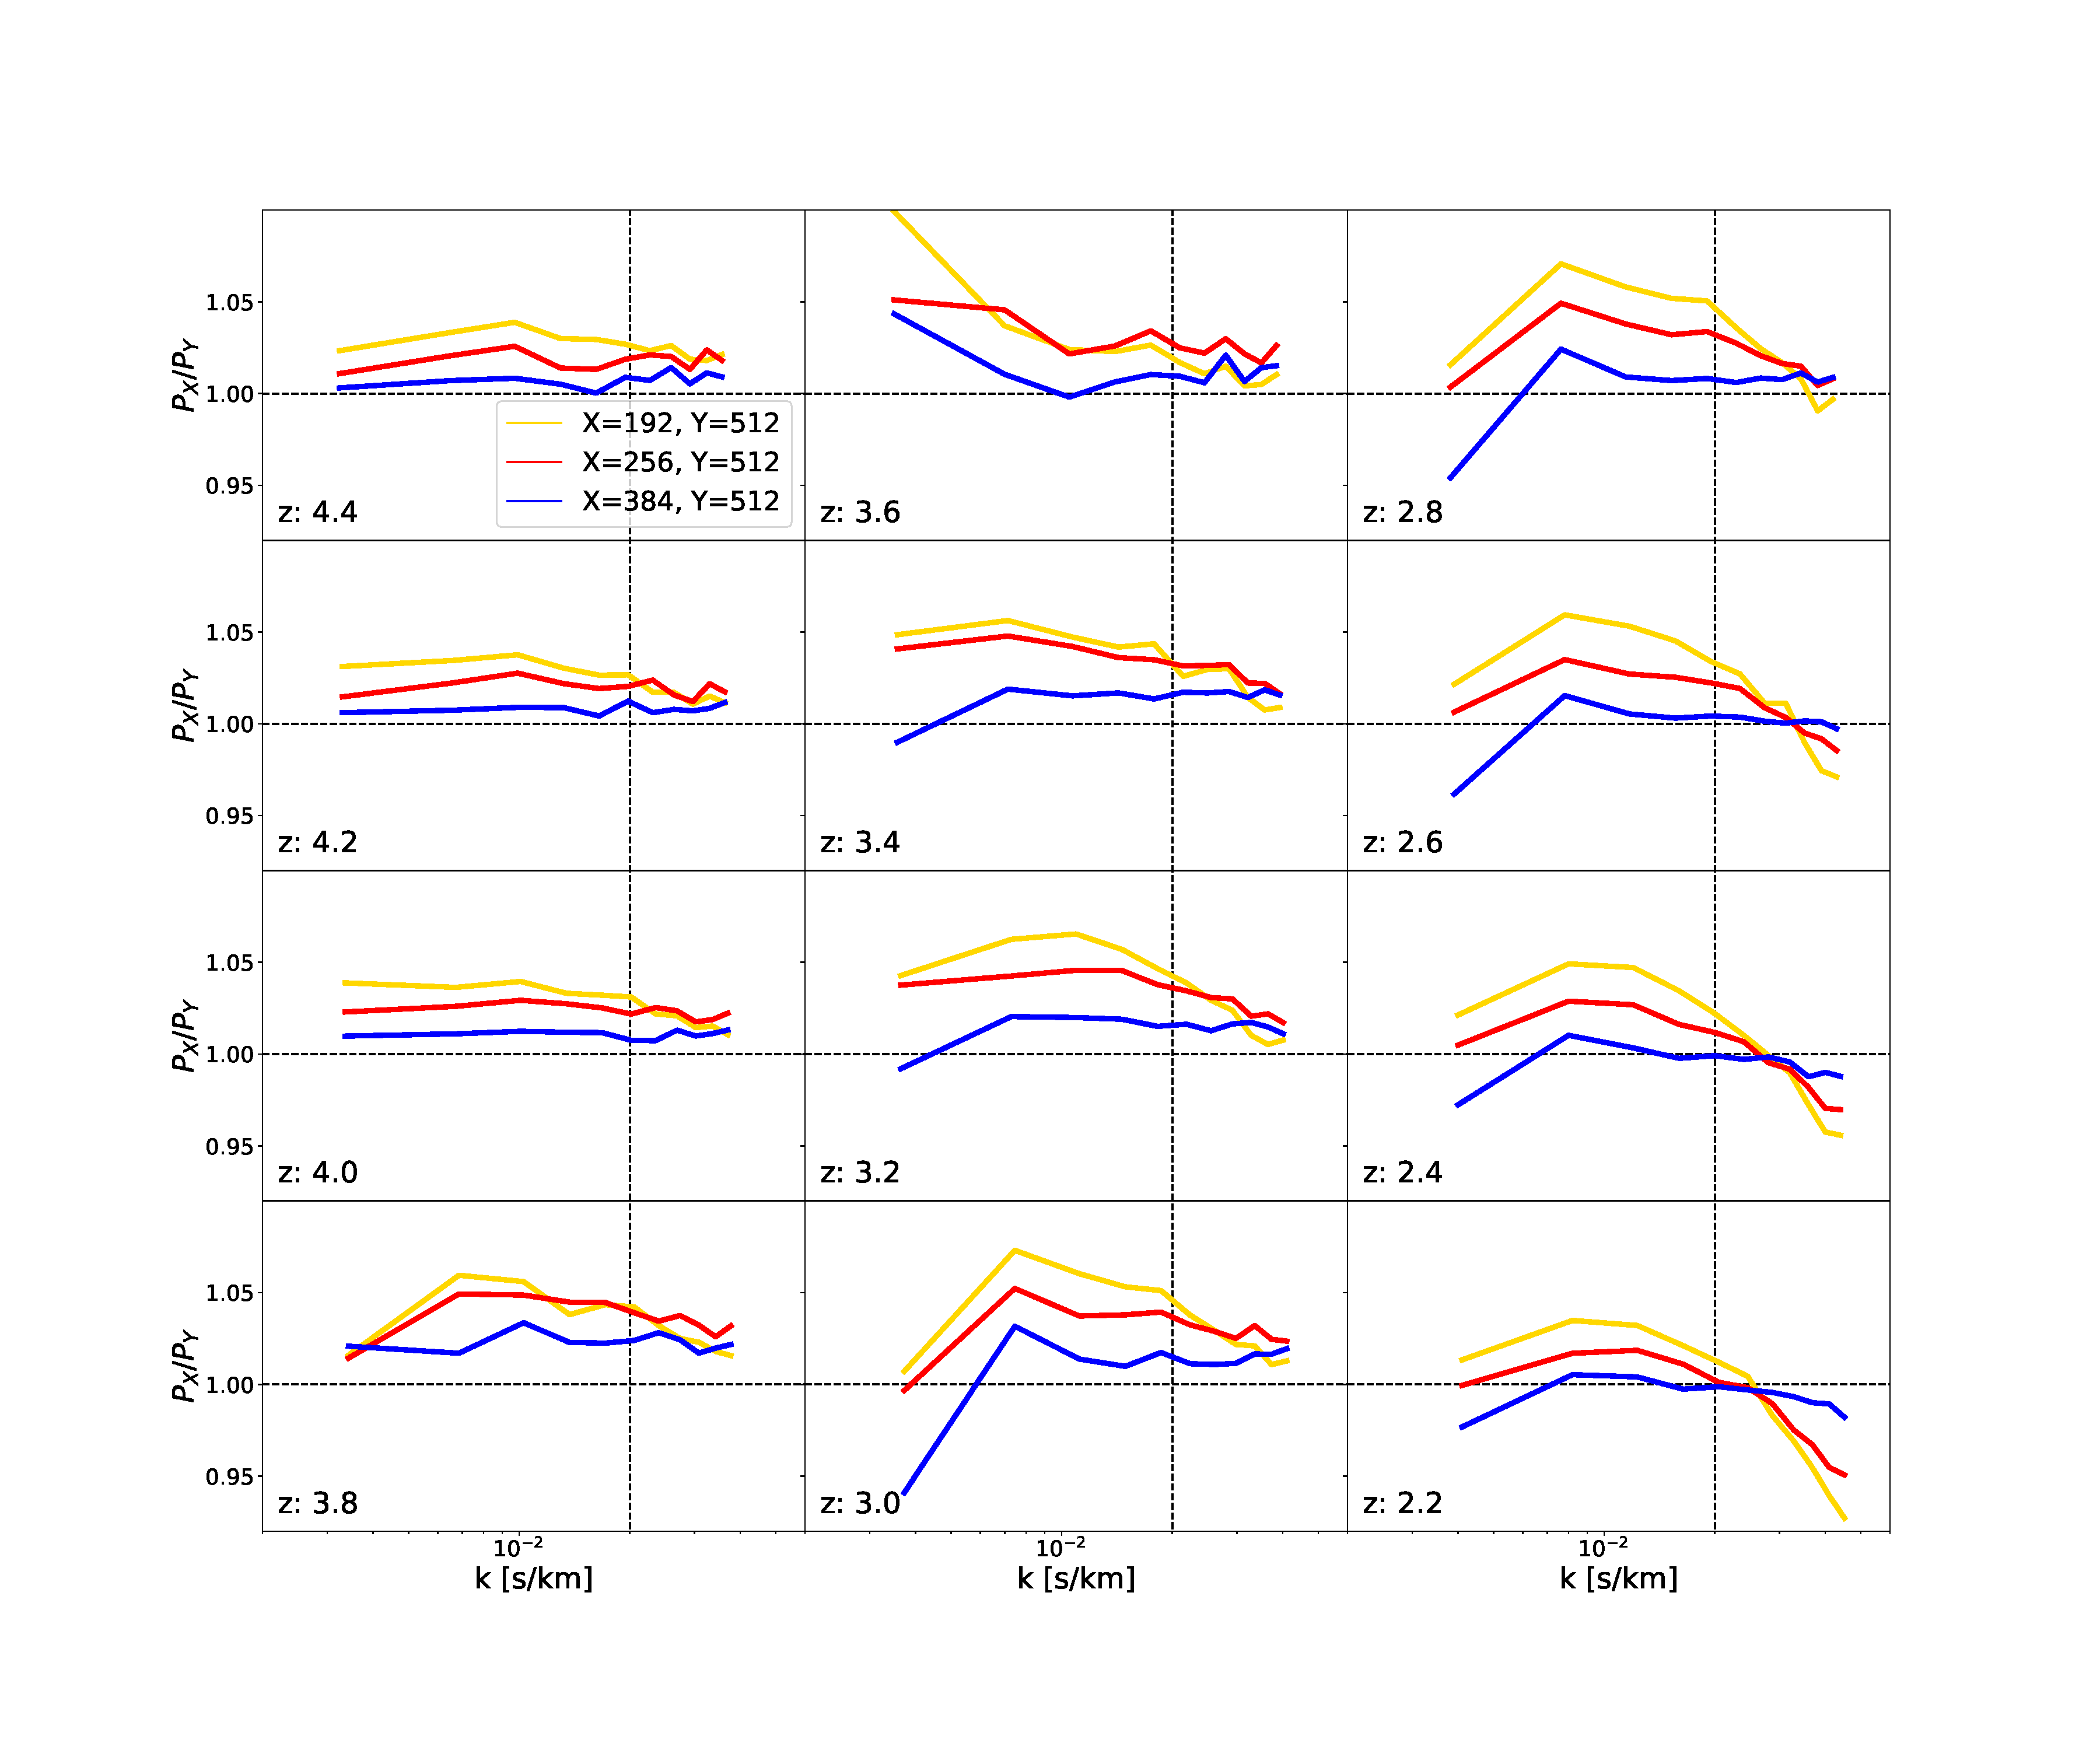
\includegraphics[width=\columnwidth]{figures/fps_mfr.pdf}
    \caption{Effect of changing each simulation parameter on the 1D flux power spectrum at $z=2$ and $z=3$. Plots should look a bit like Figure 9 of \url{https://arxiv.org/pdf/1401.6472.pdf}. Each panel should have 5 lines. Let's have $9$ panels, 1 for each parameter. cosmology parameters ($n_s$, $A_s$, $\Omega_m h^2$, $h$). reionization parameters ($He_i$ and $He_f$, $\alpha_q$, $HI_z$). Finally black hole feedback. }
    \label{fig:fluxpower}
\end{figure}

\subsection{Box Size and Particle Load}
\label{sec:boxsize}

Describe the resolution and box size of the simulation. Justify this by citing the relevant 2014 paper and with the figure. \spb{Note that the convergence at high redshift is a little better than Bolton and Becker 2010, because the heating effect of the ionization fronts smooths the high redshift gas and prevents the small unresolved halos from accreting anyway.}

\begin{figure*}
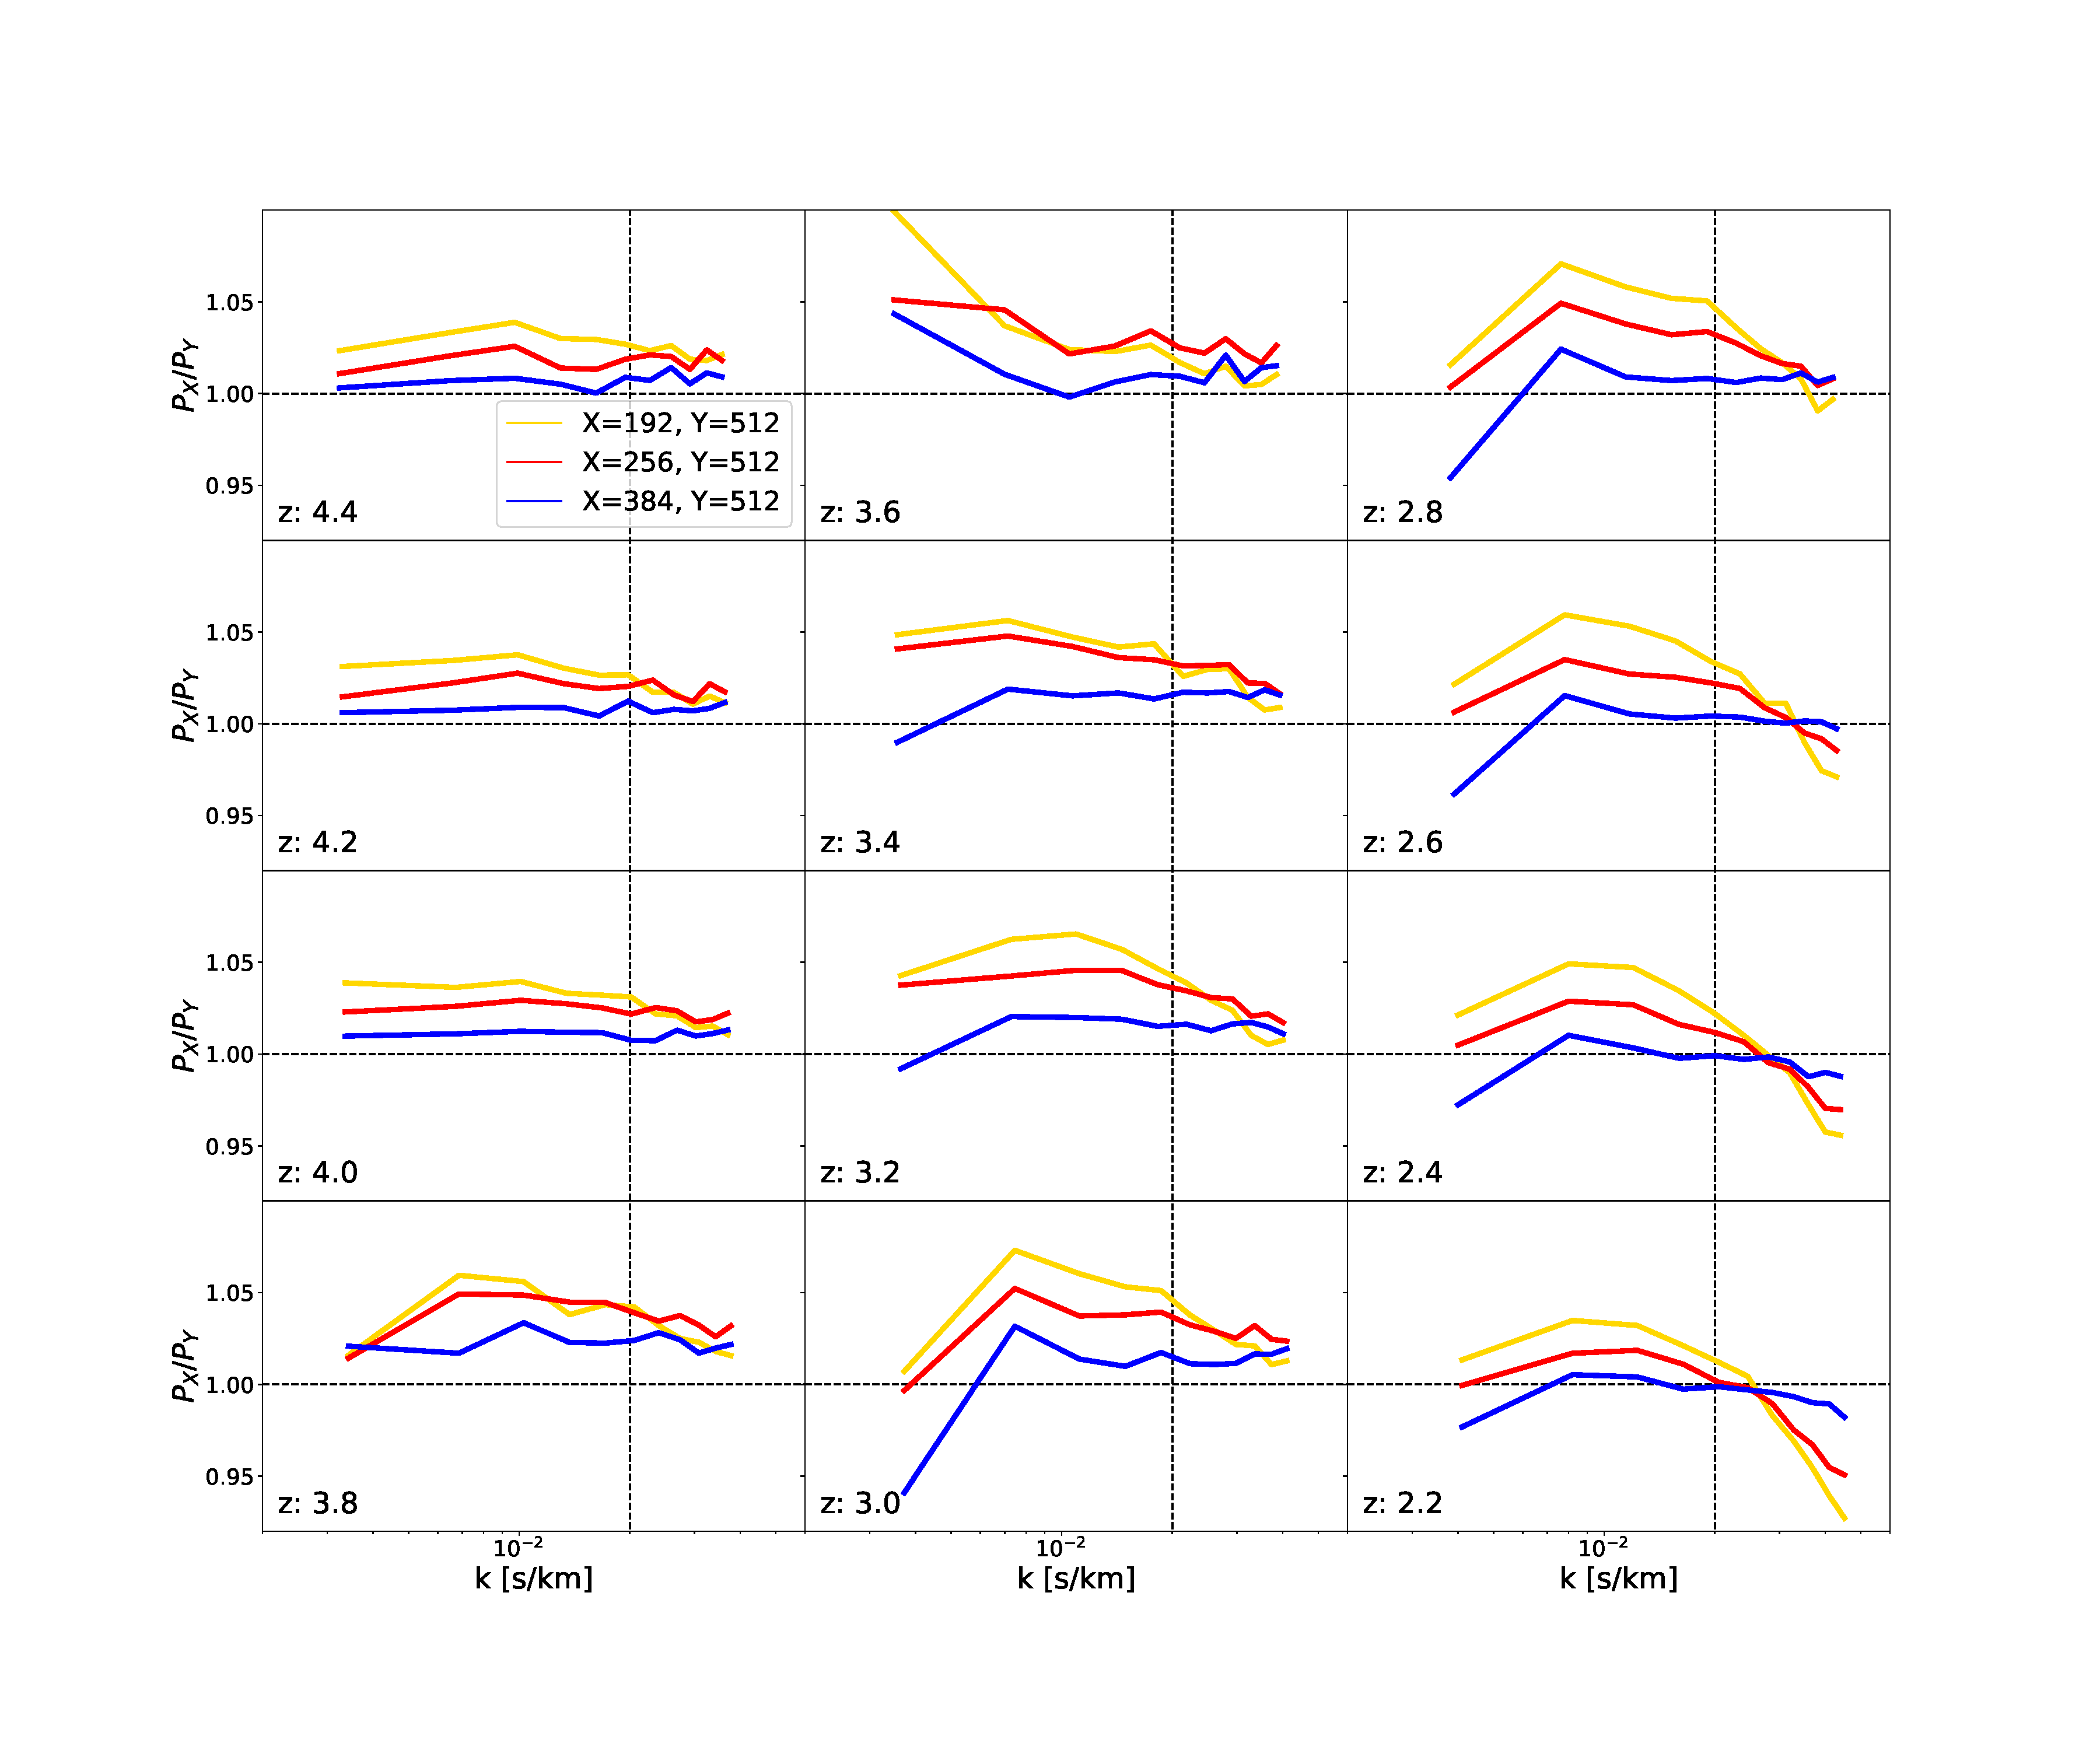
\includegraphics[width=0.45\textwidth]{figures/fps_mfr.pdf}
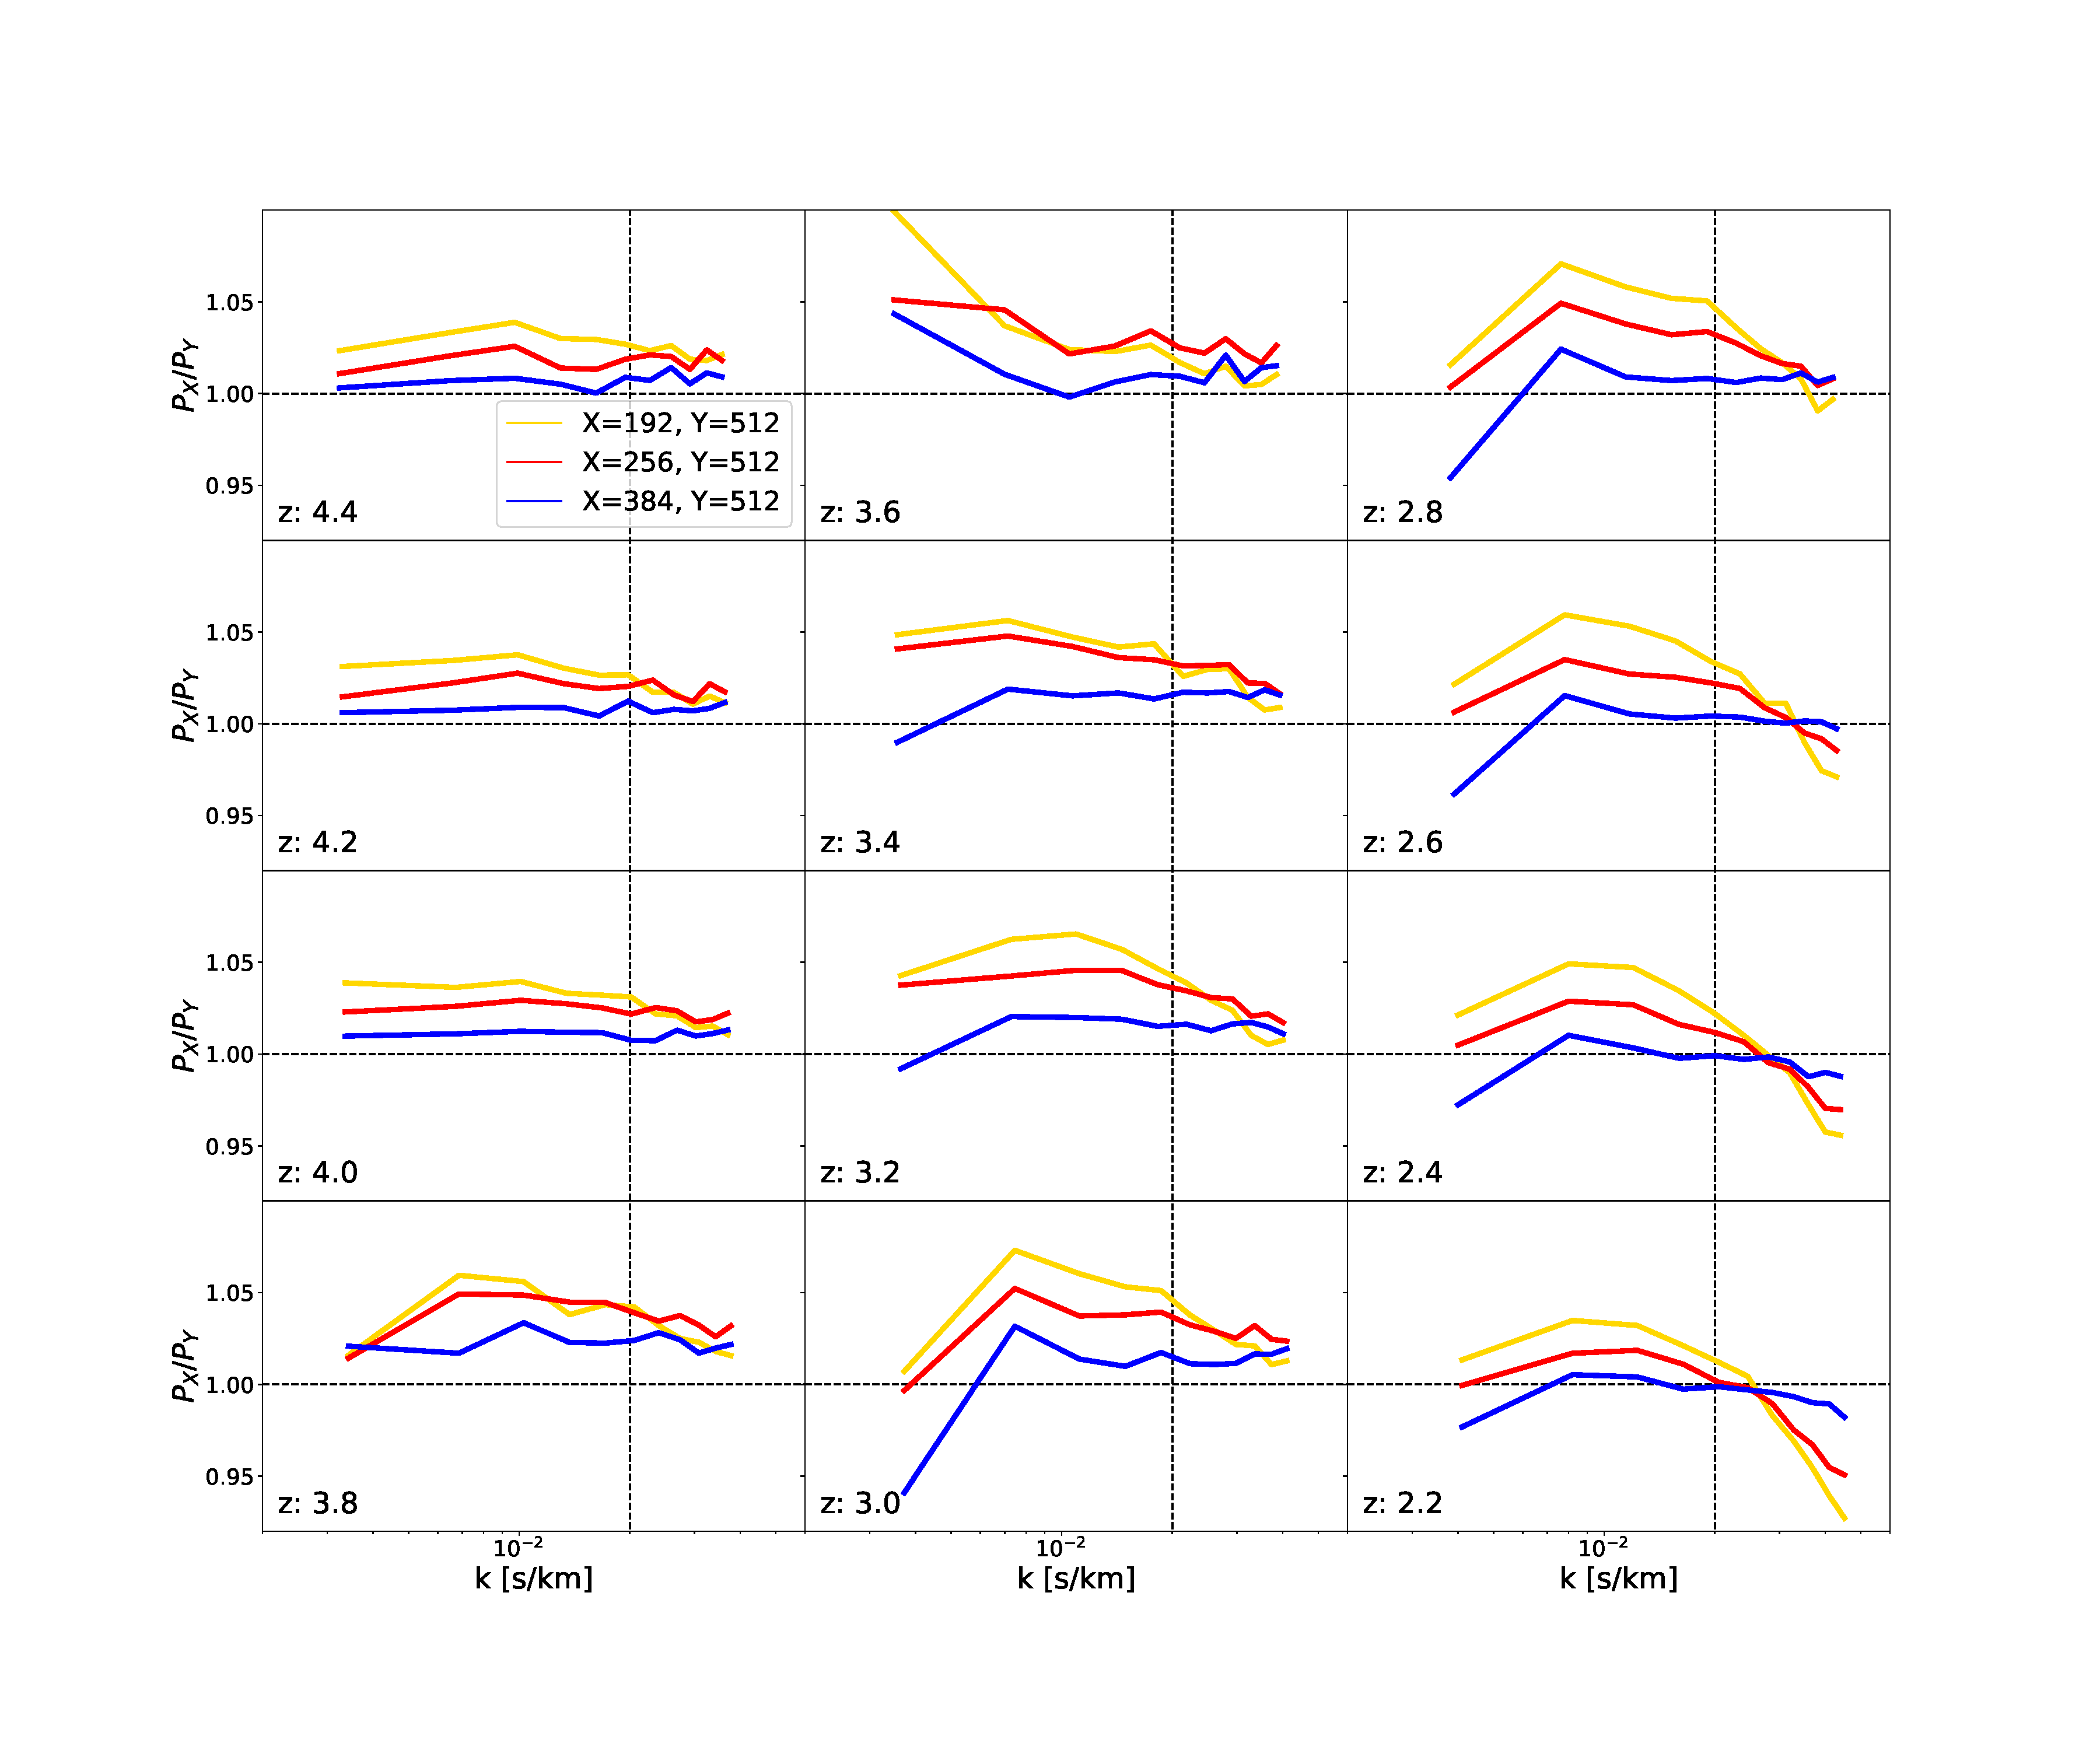
\includegraphics[width=0.45\textwidth]{figures/fps_mfr.pdf}
 \caption{Convergence of the flux power spectrum with resolution and box size. Explain box size and resolution parameters.}
 \label{fig:resolution}
\end{figure*}


\begin{figure*}
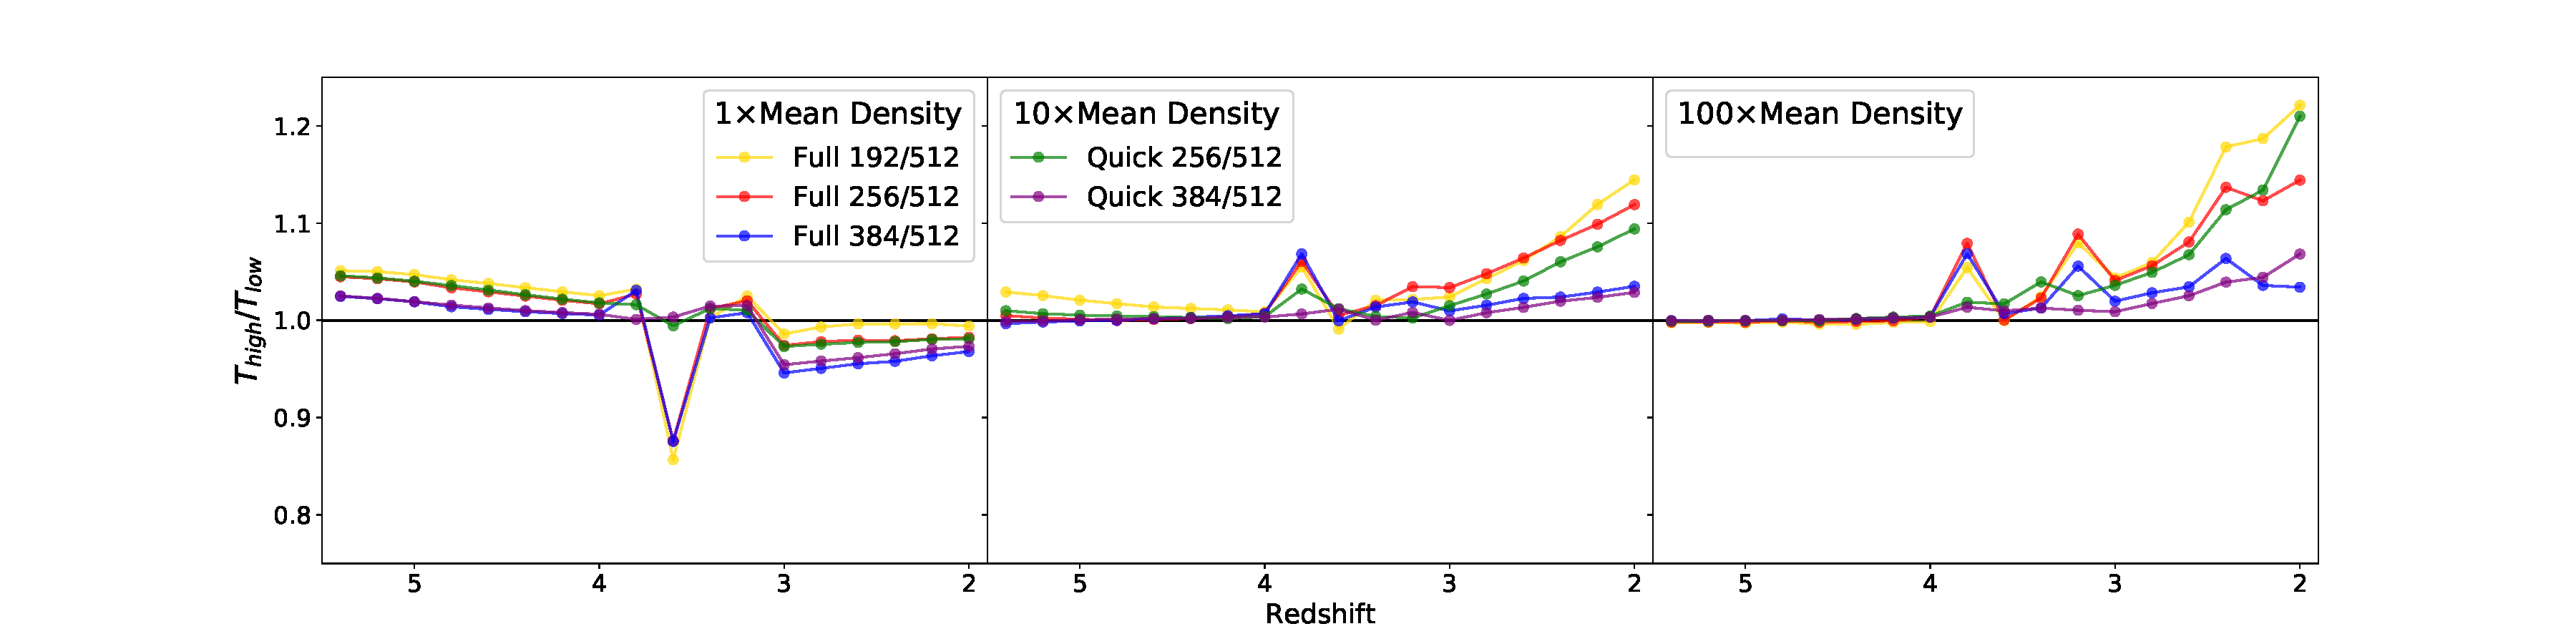
\includegraphics[width=1.\textwidth]{figures/comp-temps_fq.pdf}
 \caption{Temperature variations at different densities for different resolutions. Shows how the convergence changes with redshift.}
 \label{fig:resolutiontemp}
\end{figure*}

\subsection{Realised Thermal Histories}
\spb{Mean temperature plot for the helium reionization model parameters.}

\begin{figure*}
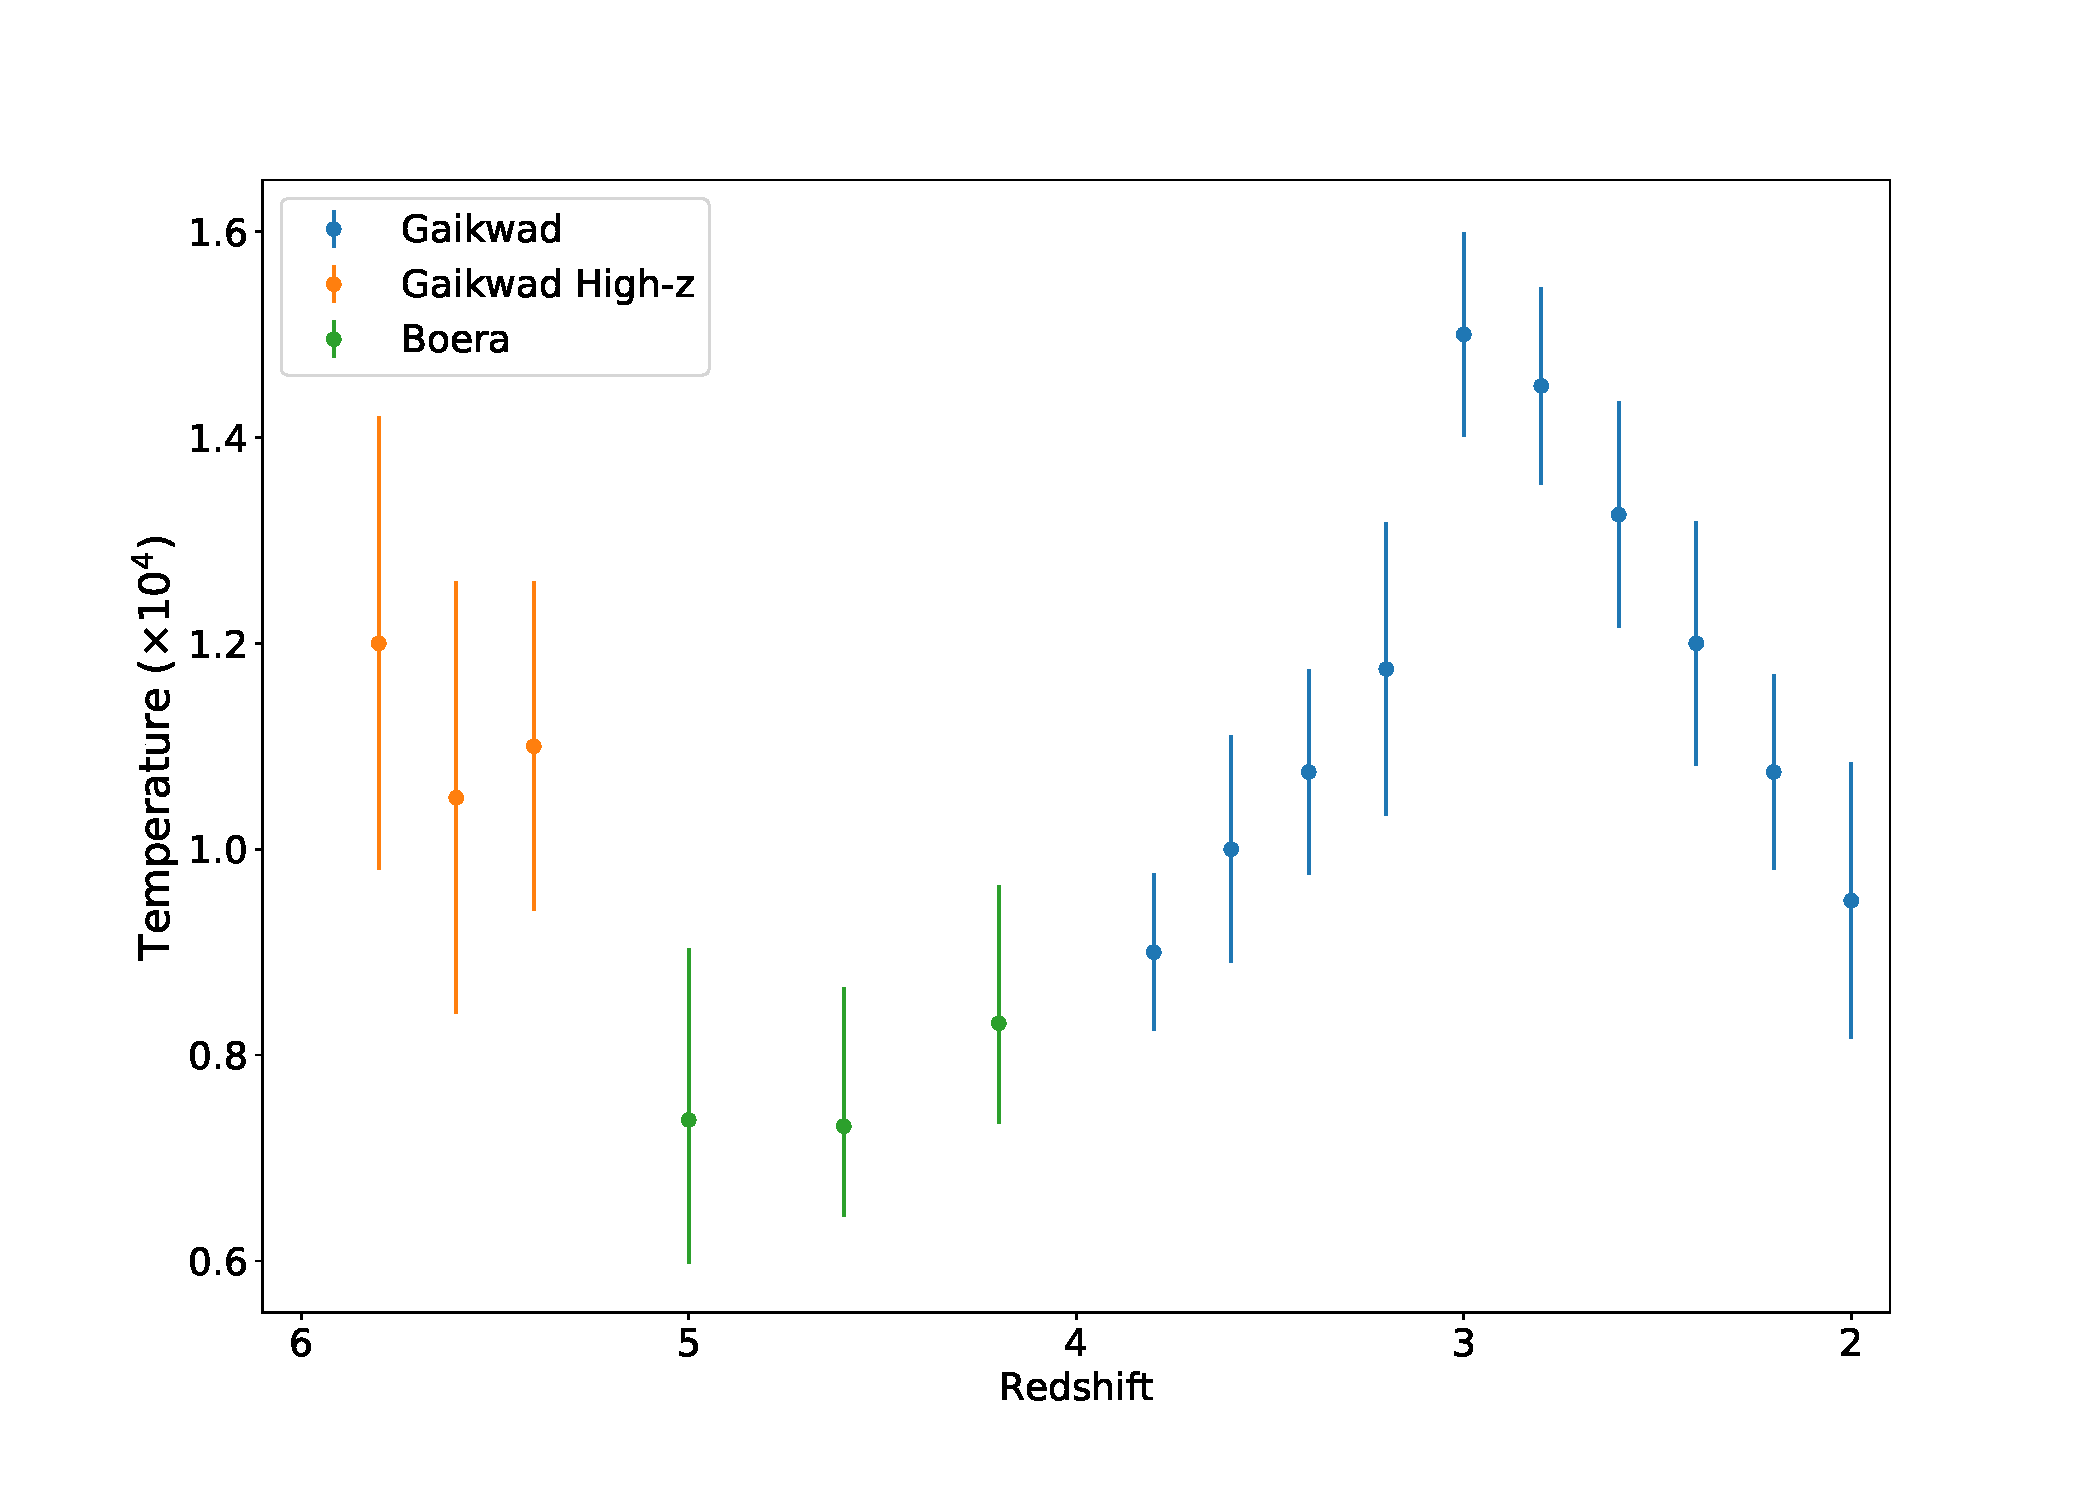
\includegraphics[width=0.45\textwidth]{figures/temp_observed.pdf}
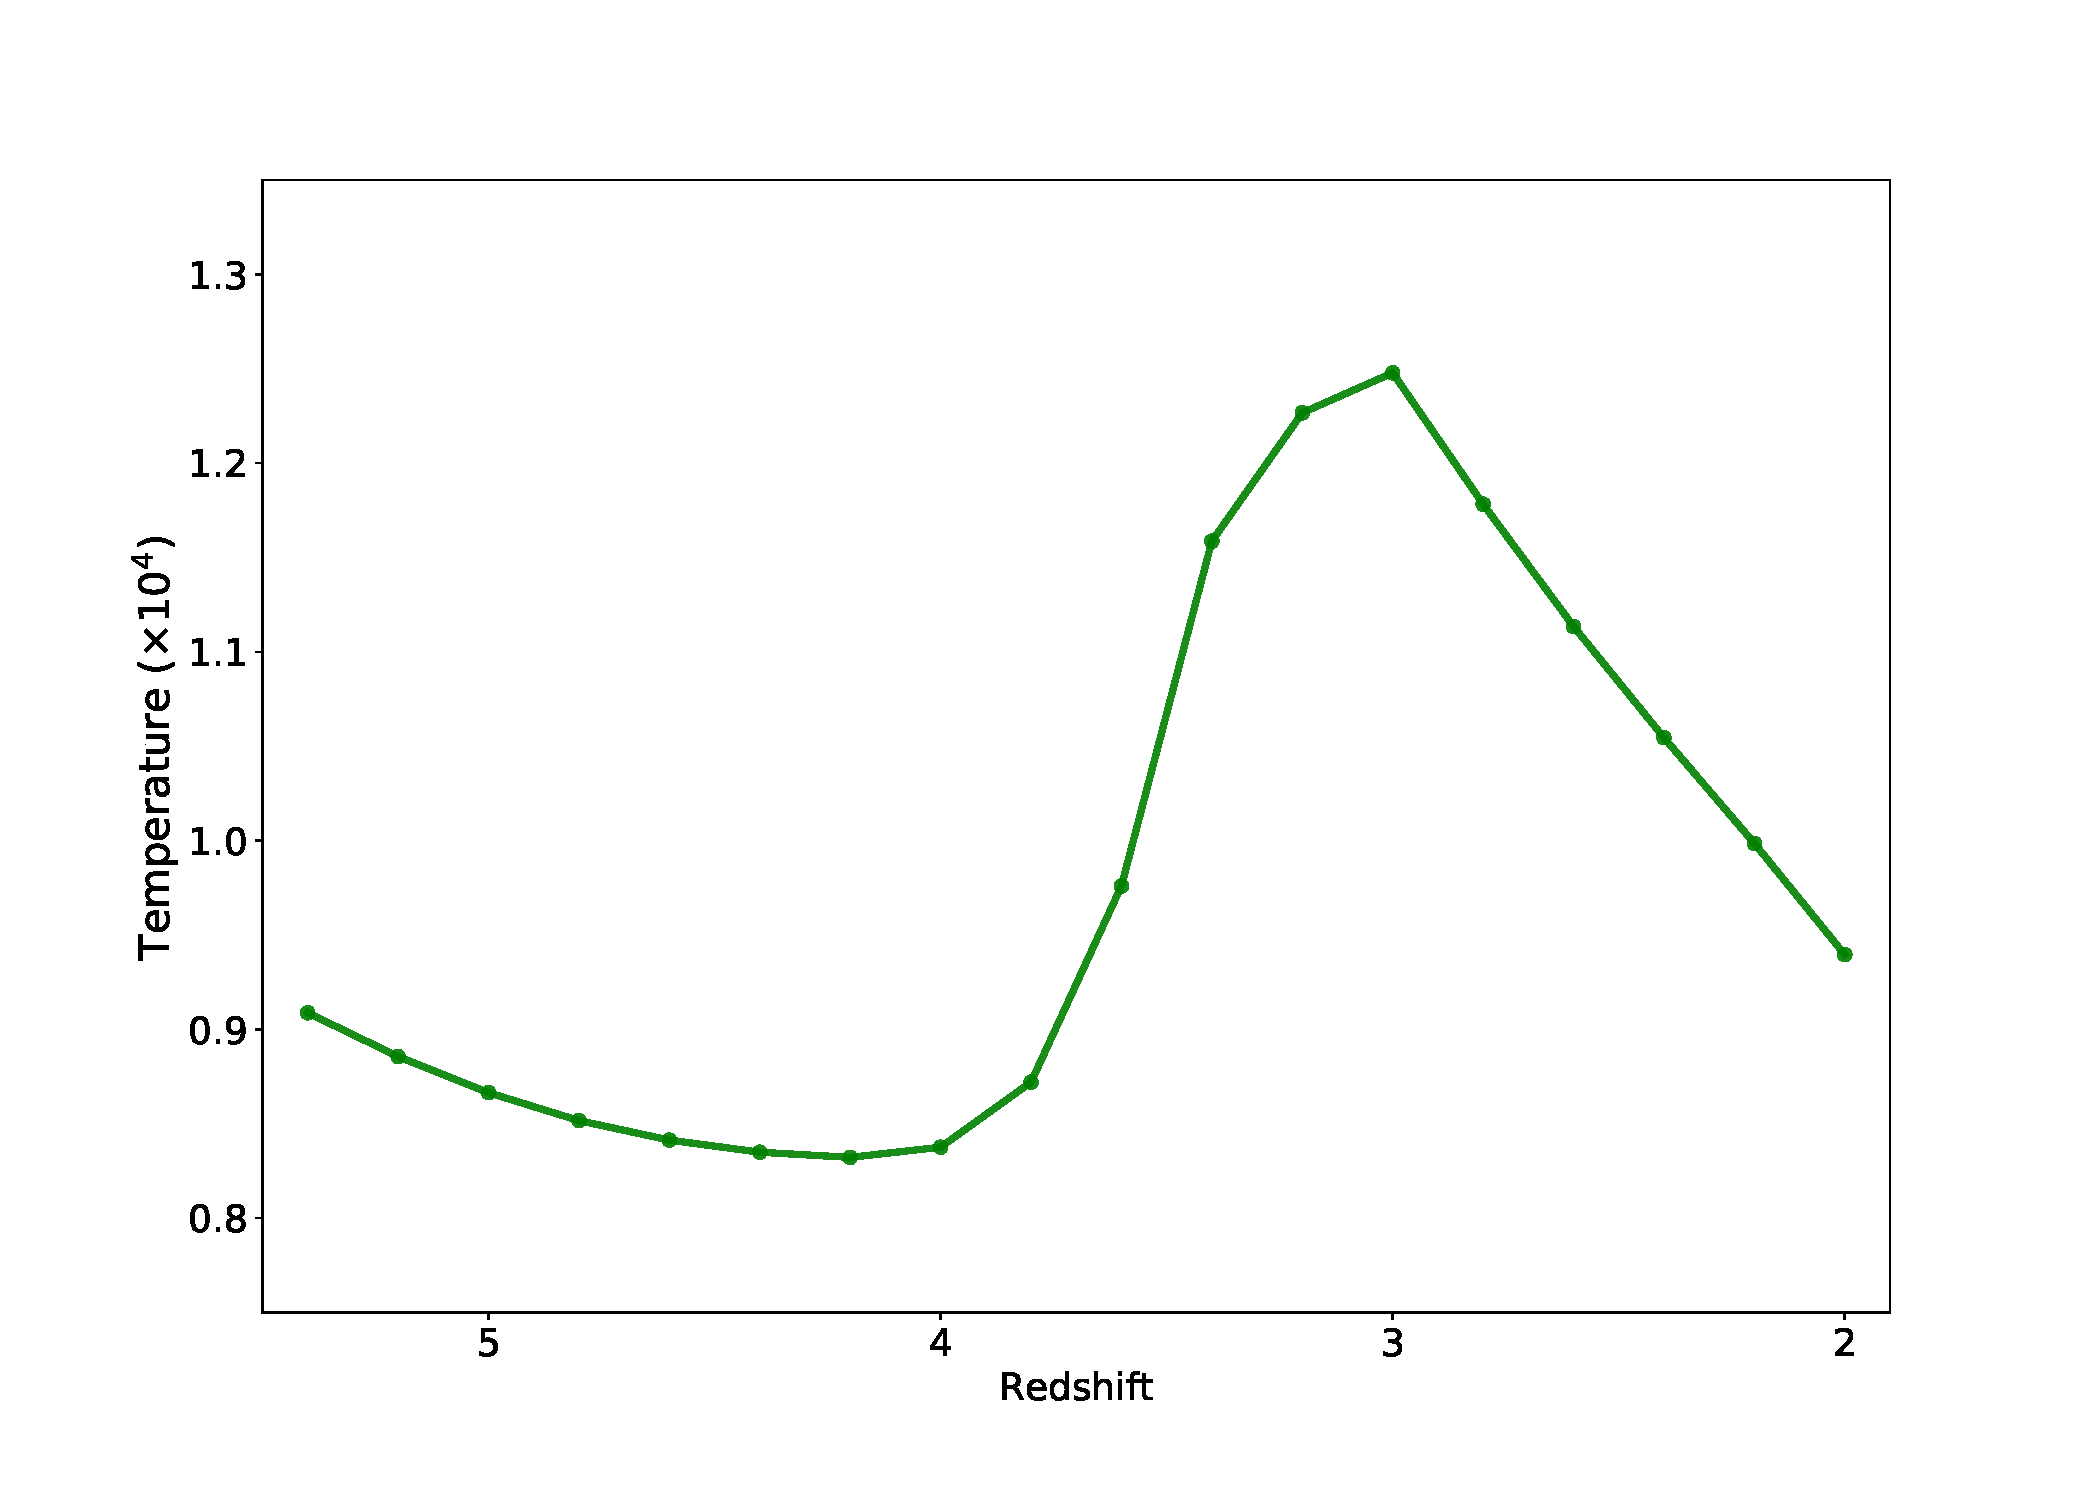
\includegraphics[width=0.45\textwidth]{figures/temps.pdf}
 \caption{Temperature at mean density as a function of redshift. One curve with the largest helium ionization starting redshift, one with the smallest. Then one with the largest $\alpha$ and one with the smallest. Put the mean temperature measurements on the same plot for comparison.}
 \label{fig:heliumtempdens}
\end{figure*}

\begin{figure*}
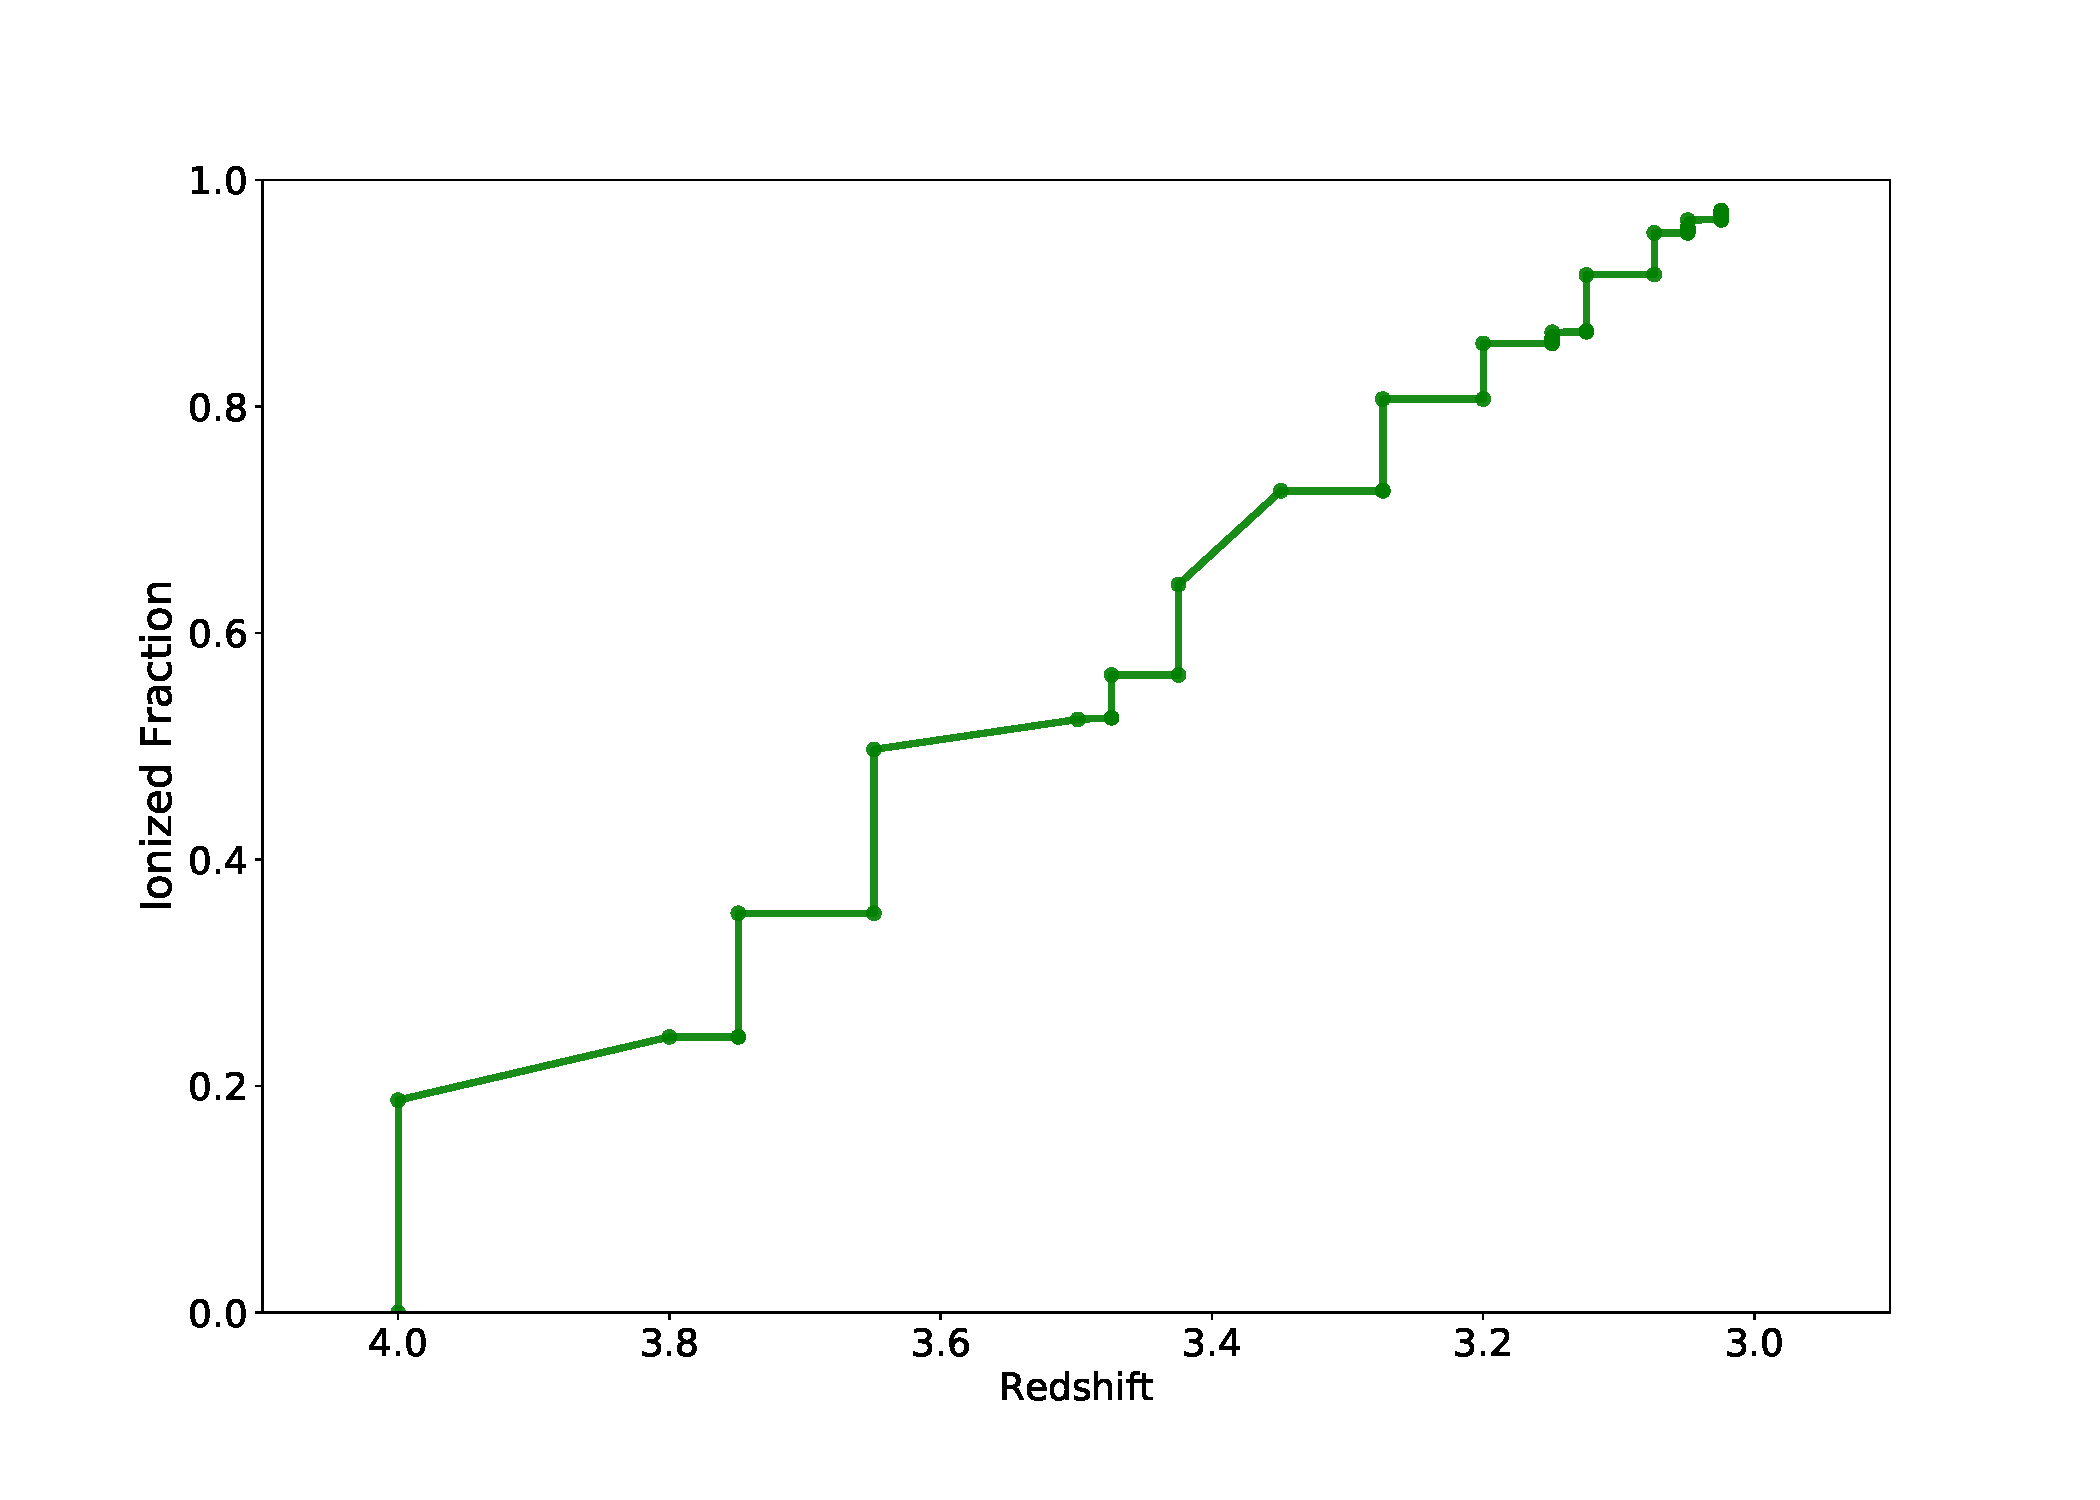
\includegraphics[width=0.45\textwidth]{figures/HeIonFrac.pdf}
 \caption{I don't think we need this one, since it will just be linear in the bigger boxes, but it would be nice to represent the information somewhere anyway for verification. Maybe a lower panel in some other figure?}
 \label{fig:heliumionizationfrac}
\end{figure*}

\begin{figure*}
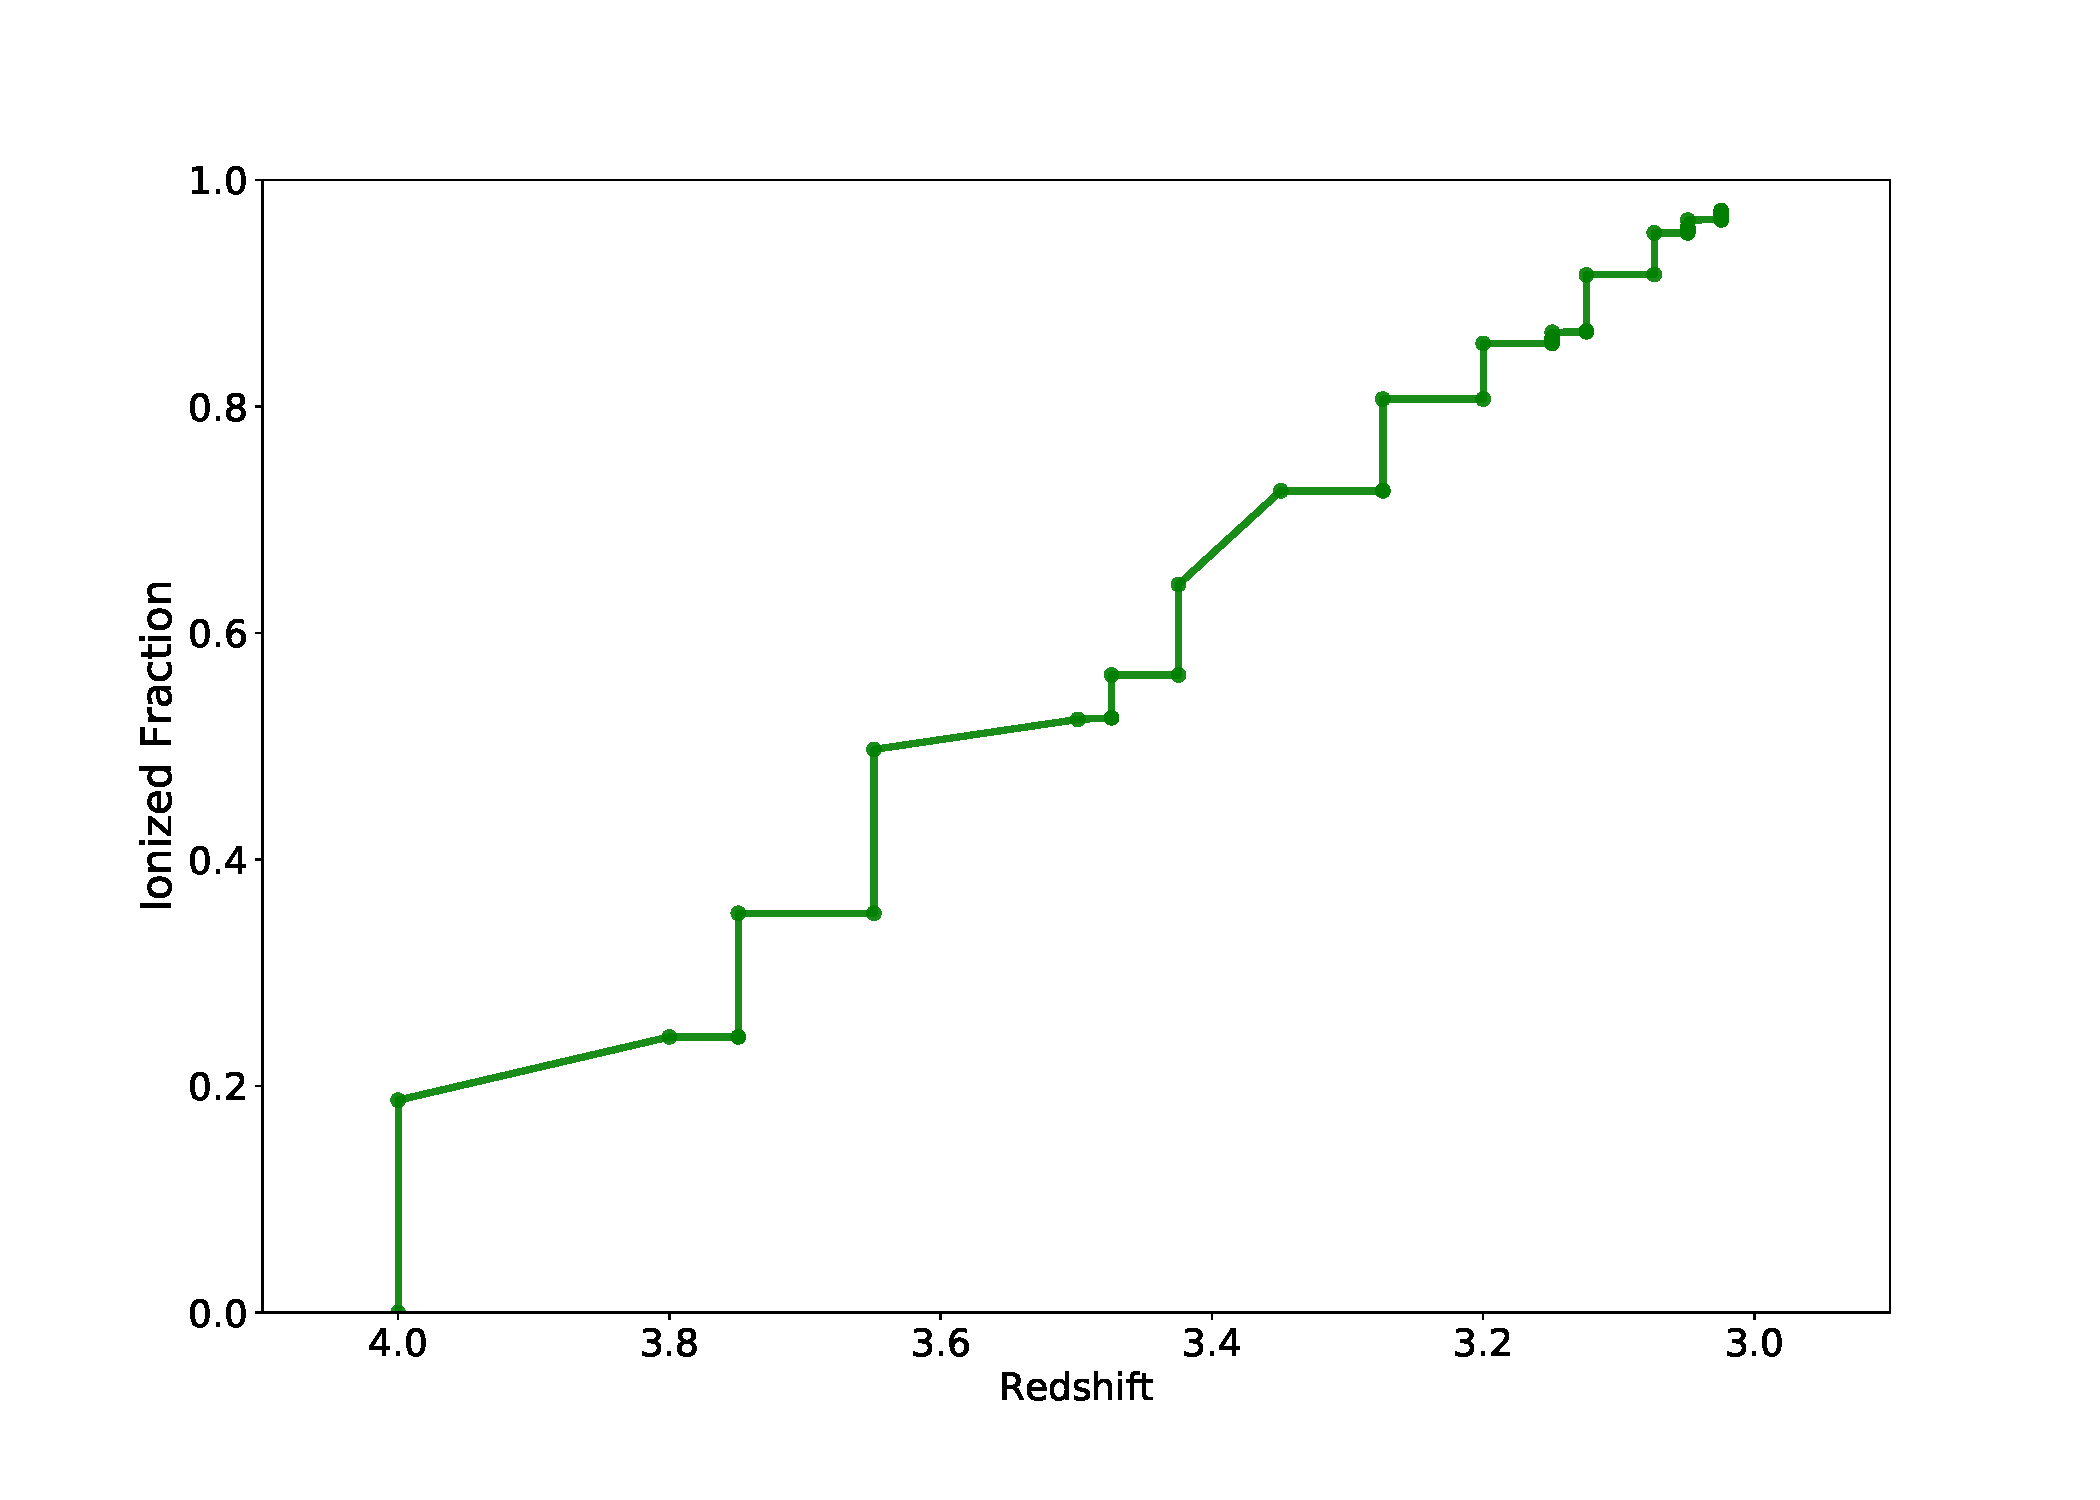
\includegraphics[width=0.45\textwidth]{figures/HeIonFrac.pdf}
 \caption{Show the temperature at mean density for different redshifts of hydrogen reionization. The point is that it has a small ish effect once we get to lower redshifts.}
 \label{fig:hydrogentempdens}
\end{figure*}

\section{Conclusion}

Mention multi-fidelity.

\section*{Acknowledgements}
MAF is supported by a National Science Foundation Graduate Research Fellowship under grant No. DGE-1326120.
MFH is supported by a National Aeronautics and Space Administration FINESST under grant No. ASTRO20-0022.
SB is supported by NSF grant AST-1817256.

Computing resources were provided by Frontera LRAC AST21005.
The authors acknowledge the Frontera computing project at the Texas Advanced Computing Center (TACC) for providing HPC and storage resources that have contributed to the research results reported within this paper.
Frontera is made possible by National Science Foundation award OAC-1818253.
URL: \url{http://www.tacc.utexas.edu}

\section*{Data Availability}
Flux power spectra generated from the low resolution, high resolution, and testing sets are available at.
Both HDF5 and plain text (appropriate for multi-fidelity emulation) formats are available.
Single- and multi-fidelity emulator predictions for the $10$ testing simulations are also available from the same repository.
The spectra underlying the flux power are available upon request.
\spb{We should try to make the spectra and flux power available for this one, but only after the likelihood paper is written.}

\bibliographystyle{JHEP}
\bibliography{refs}

\appendix

\label{lastpage}
\end{document}
